\chapter[BER Performance and Discussion]{End-to-End BER Performance and Discussion}
\label{chap:ber_results}

Chapter 4 established that the four timing estimators differ in exact-boundary accuracy, CP-safe window placement and the distribution of timing errors. This chapter examines the consequences of those errors for data detection, addressing the fourth research question. Unlike the imposed displacements in EXP02, the FFT-window positions in EXP08 are determined by the actual timing estimates. The comparison also considers computational requirements and the limitations of the simulation model.

\section[EXP08 Evaluation]{End-to-End Evaluation in EXP08}
EXP08 retains the frame structure, delay distribution, candidate search interval, channels and received active-frame SNR grid of EXP07, but uses its own random seed (2049) and newly generated data frames. Thus the timing observations used in this chapter come from EXP08, not from a trial-by-trial combination of EXP07 timing errors and EXP08 bit errors. The three receiver configurations defined in Section~3.8 are evaluated on the same received frame: perfect timing with the physical channel response, estimated timing with the physical channel response, and estimated timing with oracle phase compensation. The last two cases use exactly the same FFT window.

There are 88 algorithm--channel--SNR conditions and 10,000 frames per condition, giving 880,000 timing-estimation trials and 2,640,000 receiver evaluations. All timing estimates and receiver evaluations are valid in the saved outputs. Each receiver-specific condition therefore contains 1,280,000 decoded bits, with no observed lost bits. The cumulative count is 337,920,000 decoded bits across receiver evaluations; it is not a count of independent bit observations. Because no frames are lost, conditional BER and bit-delivery failure ratio coincide in this experiment. A valid decoded frame may nevertheless contain incorrect bits.

All empirical BER values reported here use the actual bit-error counts. The original MATLAB logarithmic plots display zero-error observations at $1/1{,}280{,}000=7.8125\times10^{-7}$ with downward triangles. This is a graphical convention, not a physical error floor, a positive observed BER or a confidence bound. In particular, the marker for one observed error may have the same vertical coordinate as a zero-error marker.

\section[Perfect-Timing Reference]{Perfect-Timing BER Reference}
\label{sec:ch5perfect}
Figure~\ref{fig:ch5perfect} shows the performance when the useful data-symbol boundary is known. This reference removes synchronization error while retaining channel effects, noise and the same data processing as the estimated-timing receivers.

\begin{figure}[!htbp]
\centering
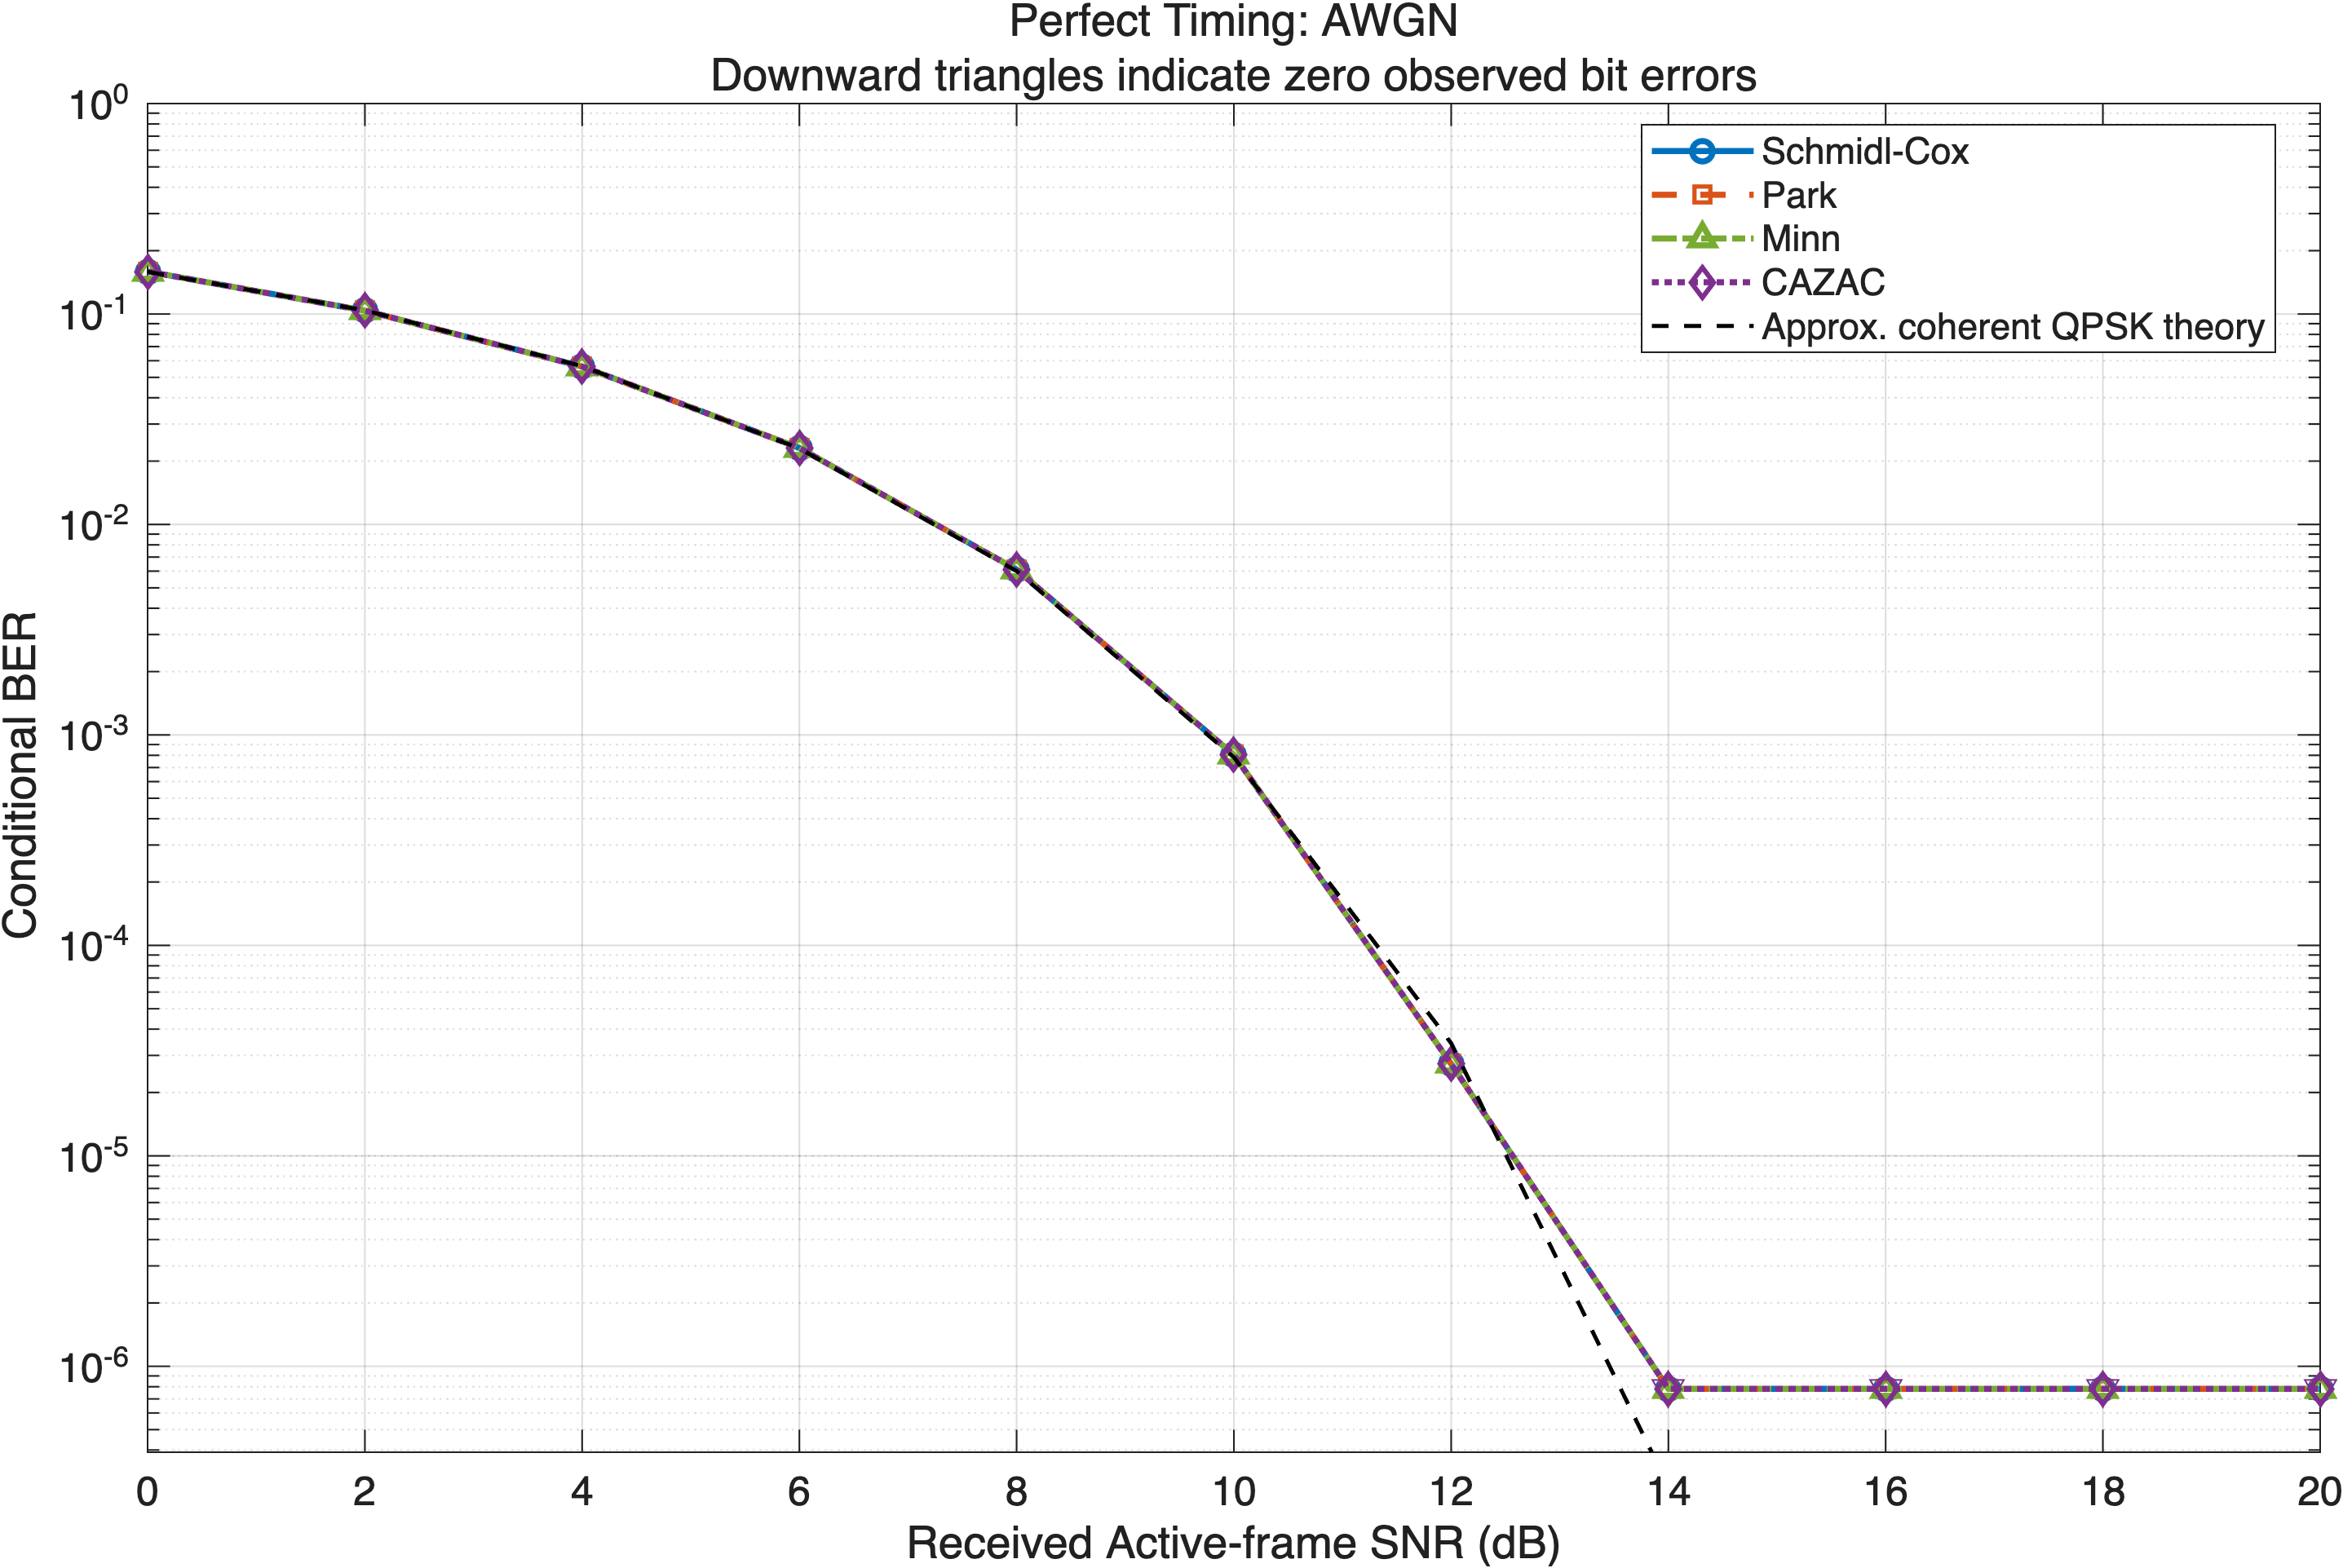
\includegraphics[width=0.90\textwidth,height=0.30\textheight,keepaspectratio]{figures/ch5/exp08_awgn_ber_perfect.png}\par
{\small (a) AWGN}\par\medskip
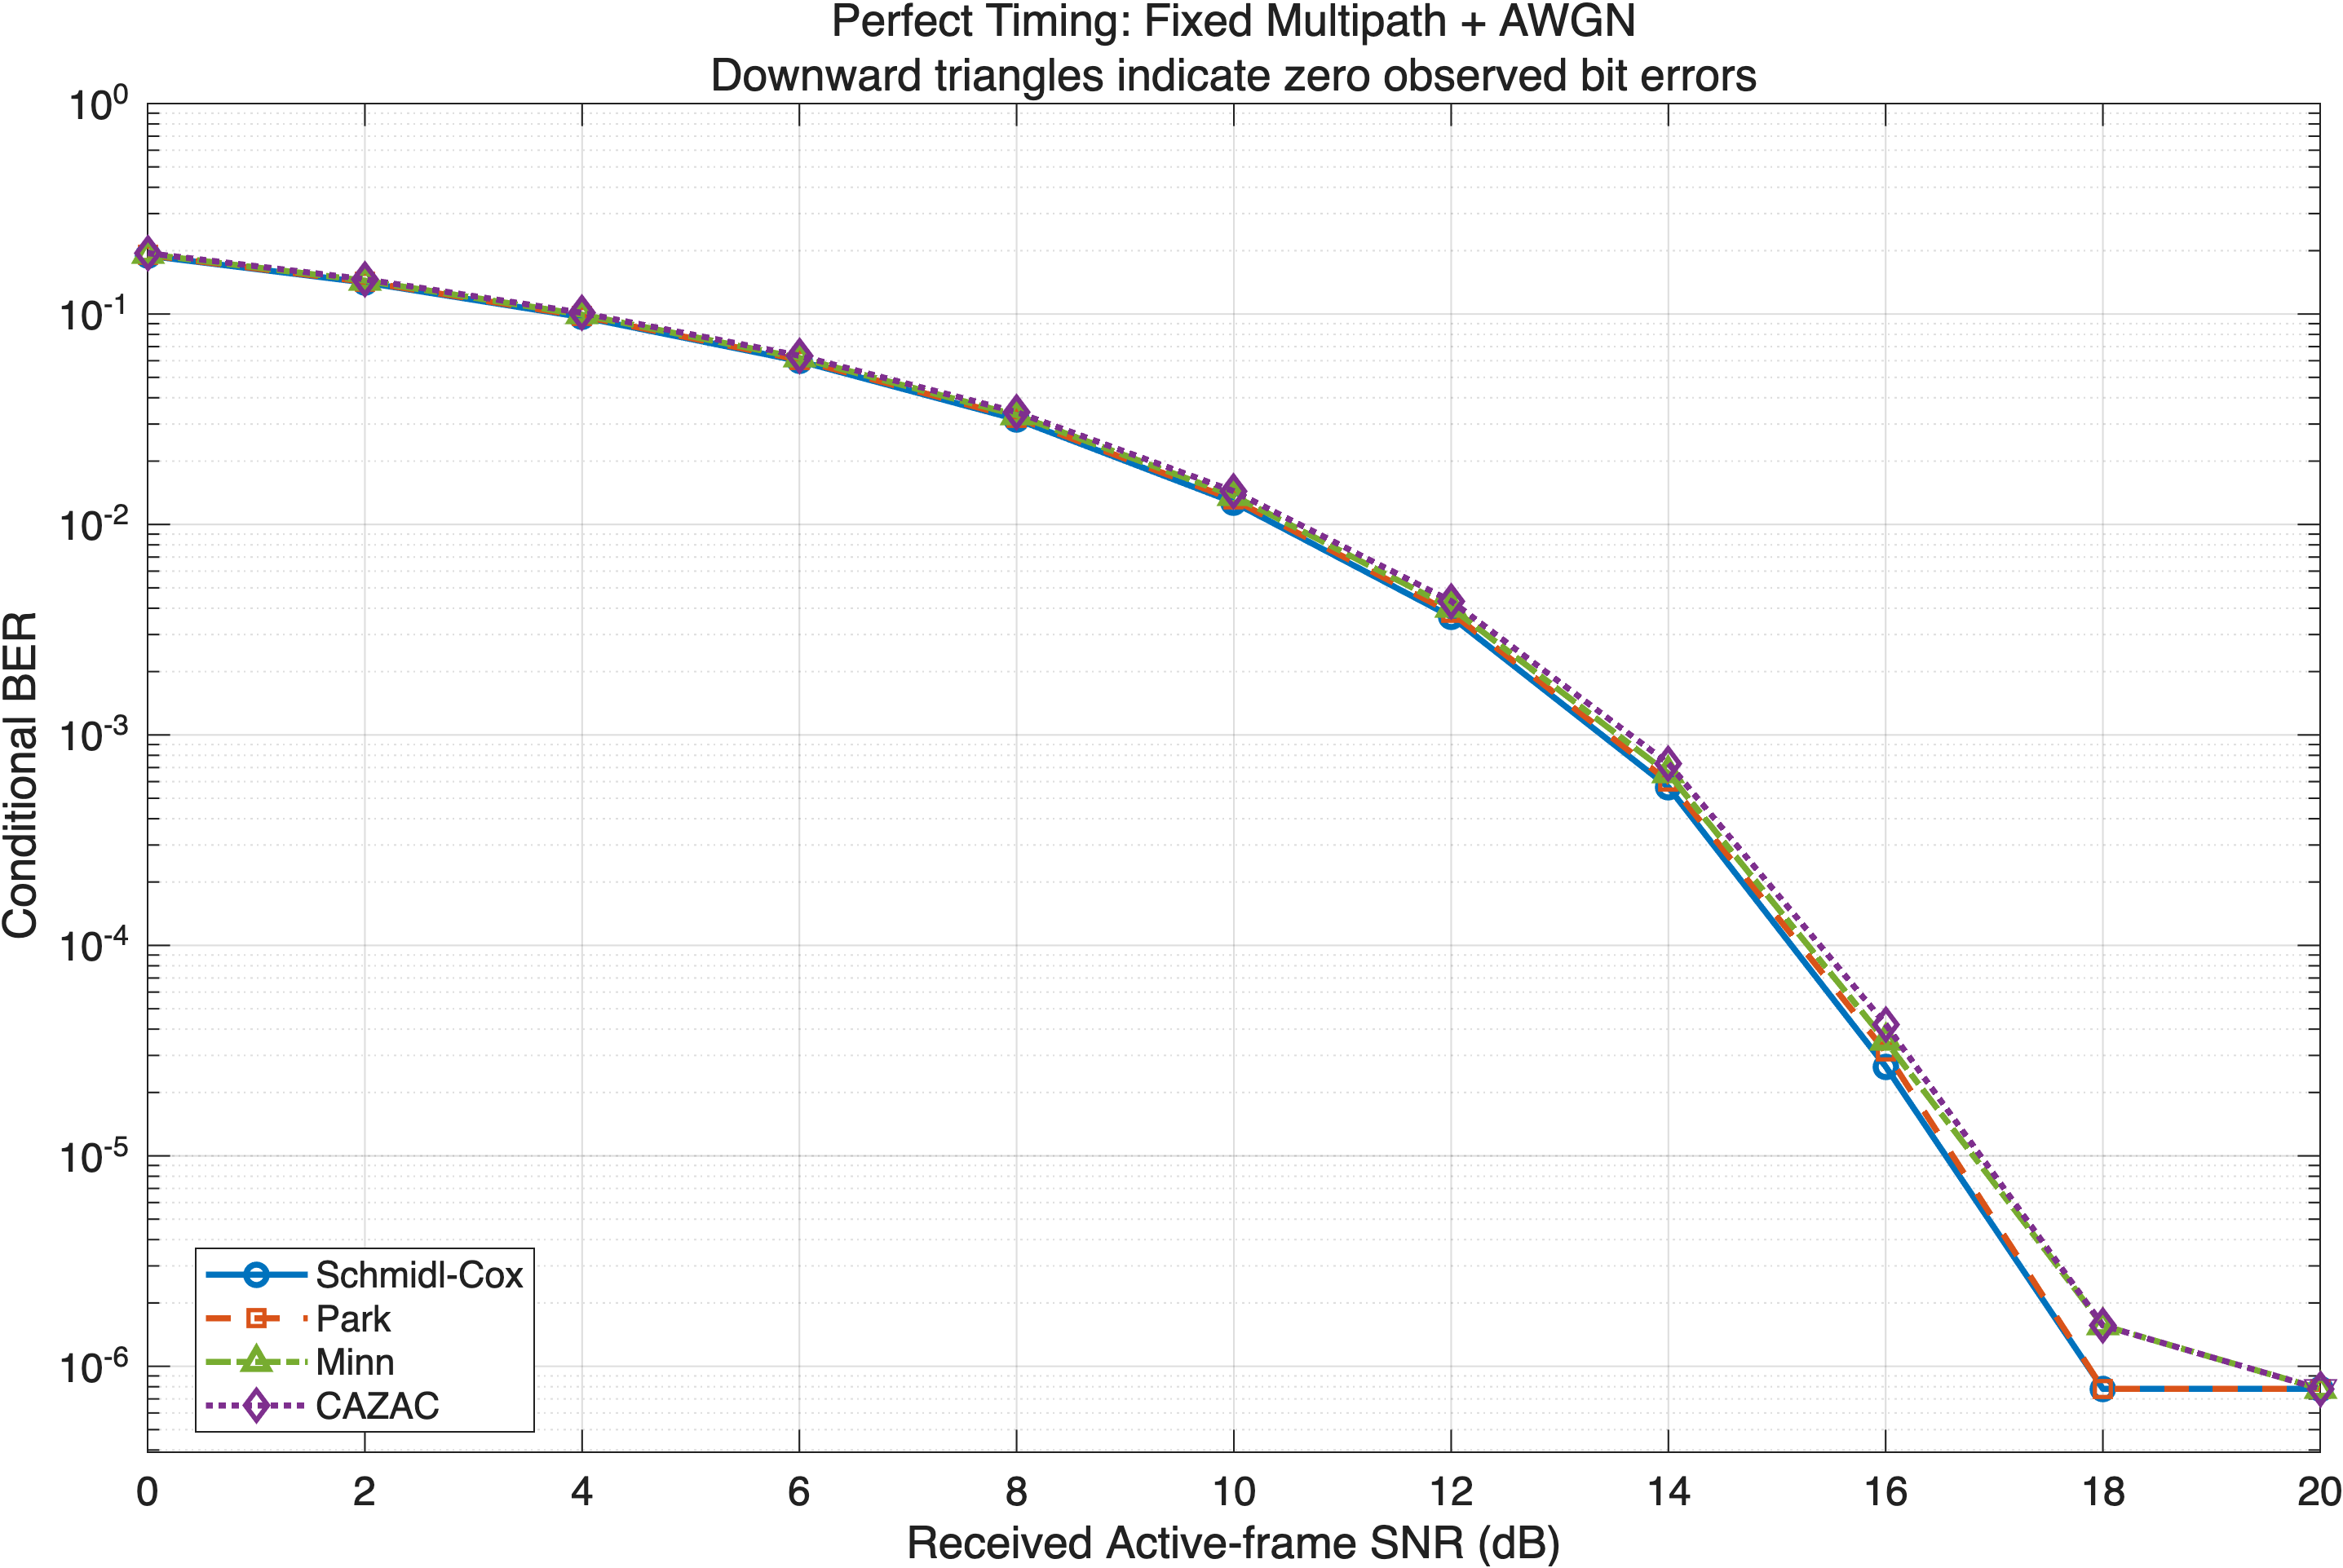
\includegraphics[width=0.90\textwidth,height=0.30\textheight,keepaspectratio]{figures/ch5/exp08_multipath_ber_perfect.png}\par
{\small (b) Fixed multipath with AWGN}
\caption[EXP08: perfect-timing BER.]{EXP08: BER with perfect timing. Downward triangles denote zero observed bit errors.}
\label{fig:ch5perfect}
\end{figure}

In AWGN, all four perfect-timing curves coincide. For a given trial, the same data vector and base noise are used, and every training and data symbol has the same CP-inclusive energy. The received active-frame power is therefore one in AWGN, independently of the preamble design. At 0 dB the common reference records 203,729 bit errors (BER 0.1591633); at 10 dB it records 1,029 errors (BER 0.0008039063). No errors are observed in these reference receivers from 14 to 20 dB.

The approximate coherent QPSK curve shown in the AWGN figures is $Q(\sqrt{\gamma})$, where $\gamma=10^{\gamma_{\mathrm{dB}}/10}$ denotes the received active-frame SNR in linear units. This uses the approximation that the useful-sample SNR equals the active-frame SNR, so that $E_b/N_0\simeq\gamma/2$. The exact useful-data power may vary because the normalization includes the CP. The curve is consequently a useful reference rather than an exact analytical expression for every normalized frame. The SNR axis in EXP08 is not the useful-data $E_b/N_0$ axis of EXP01.

The multipath references have higher BER over much of the tested grid. Zero-forcing equalization removes the deterministic channel gains, but the noise variance on subcarrier $k$ is multiplied by $1/|H[k]|^2$. Under the unnormalized receiver DFT, the noise power per FFT coefficient before equalization is $N\sigma_w^2$. A channel with nonuniform $|H[k]|$ therefore produces unequal effective detection SNRs across the subcarriers.

The multipath perfect-timing curves are also slightly different among algorithms. This does not imply that one timing estimator is better when true timing is already supplied. Received active-frame powers averaged across all EXP08 multipath trials are 0.99834, 1.01012, 1.02807 and 1.05068 for S\&C, Park, Minn and CAZAC, respectively. The corresponding noise variance is calculated separately from each received frame's power, as described in Section~3.3. At 10 dB, for instance, the perfect reference BER ranges from 0.012729 for S\&C to 0.014378 for CAZAC. The appropriate synchronization comparison is therefore against each method's own perfect-timing reference.

\section[Estimated-Timing BER]{BER with Estimated Timing}
\label{sec:ch5estimated}
Figure~\ref{fig:ch5estimated} compares the four estimators when their estimated timing positions are used without residual phase compensation. Tables~\ref{tab:ch5awgn} and \ref{tab:ch5mp} give exact bit-error counts at selected SNR levels for all three receiver configurations. Dividing each entry by 1,280,000 gives the corresponding BER.

\begin{figure}[!htbp]
\centering
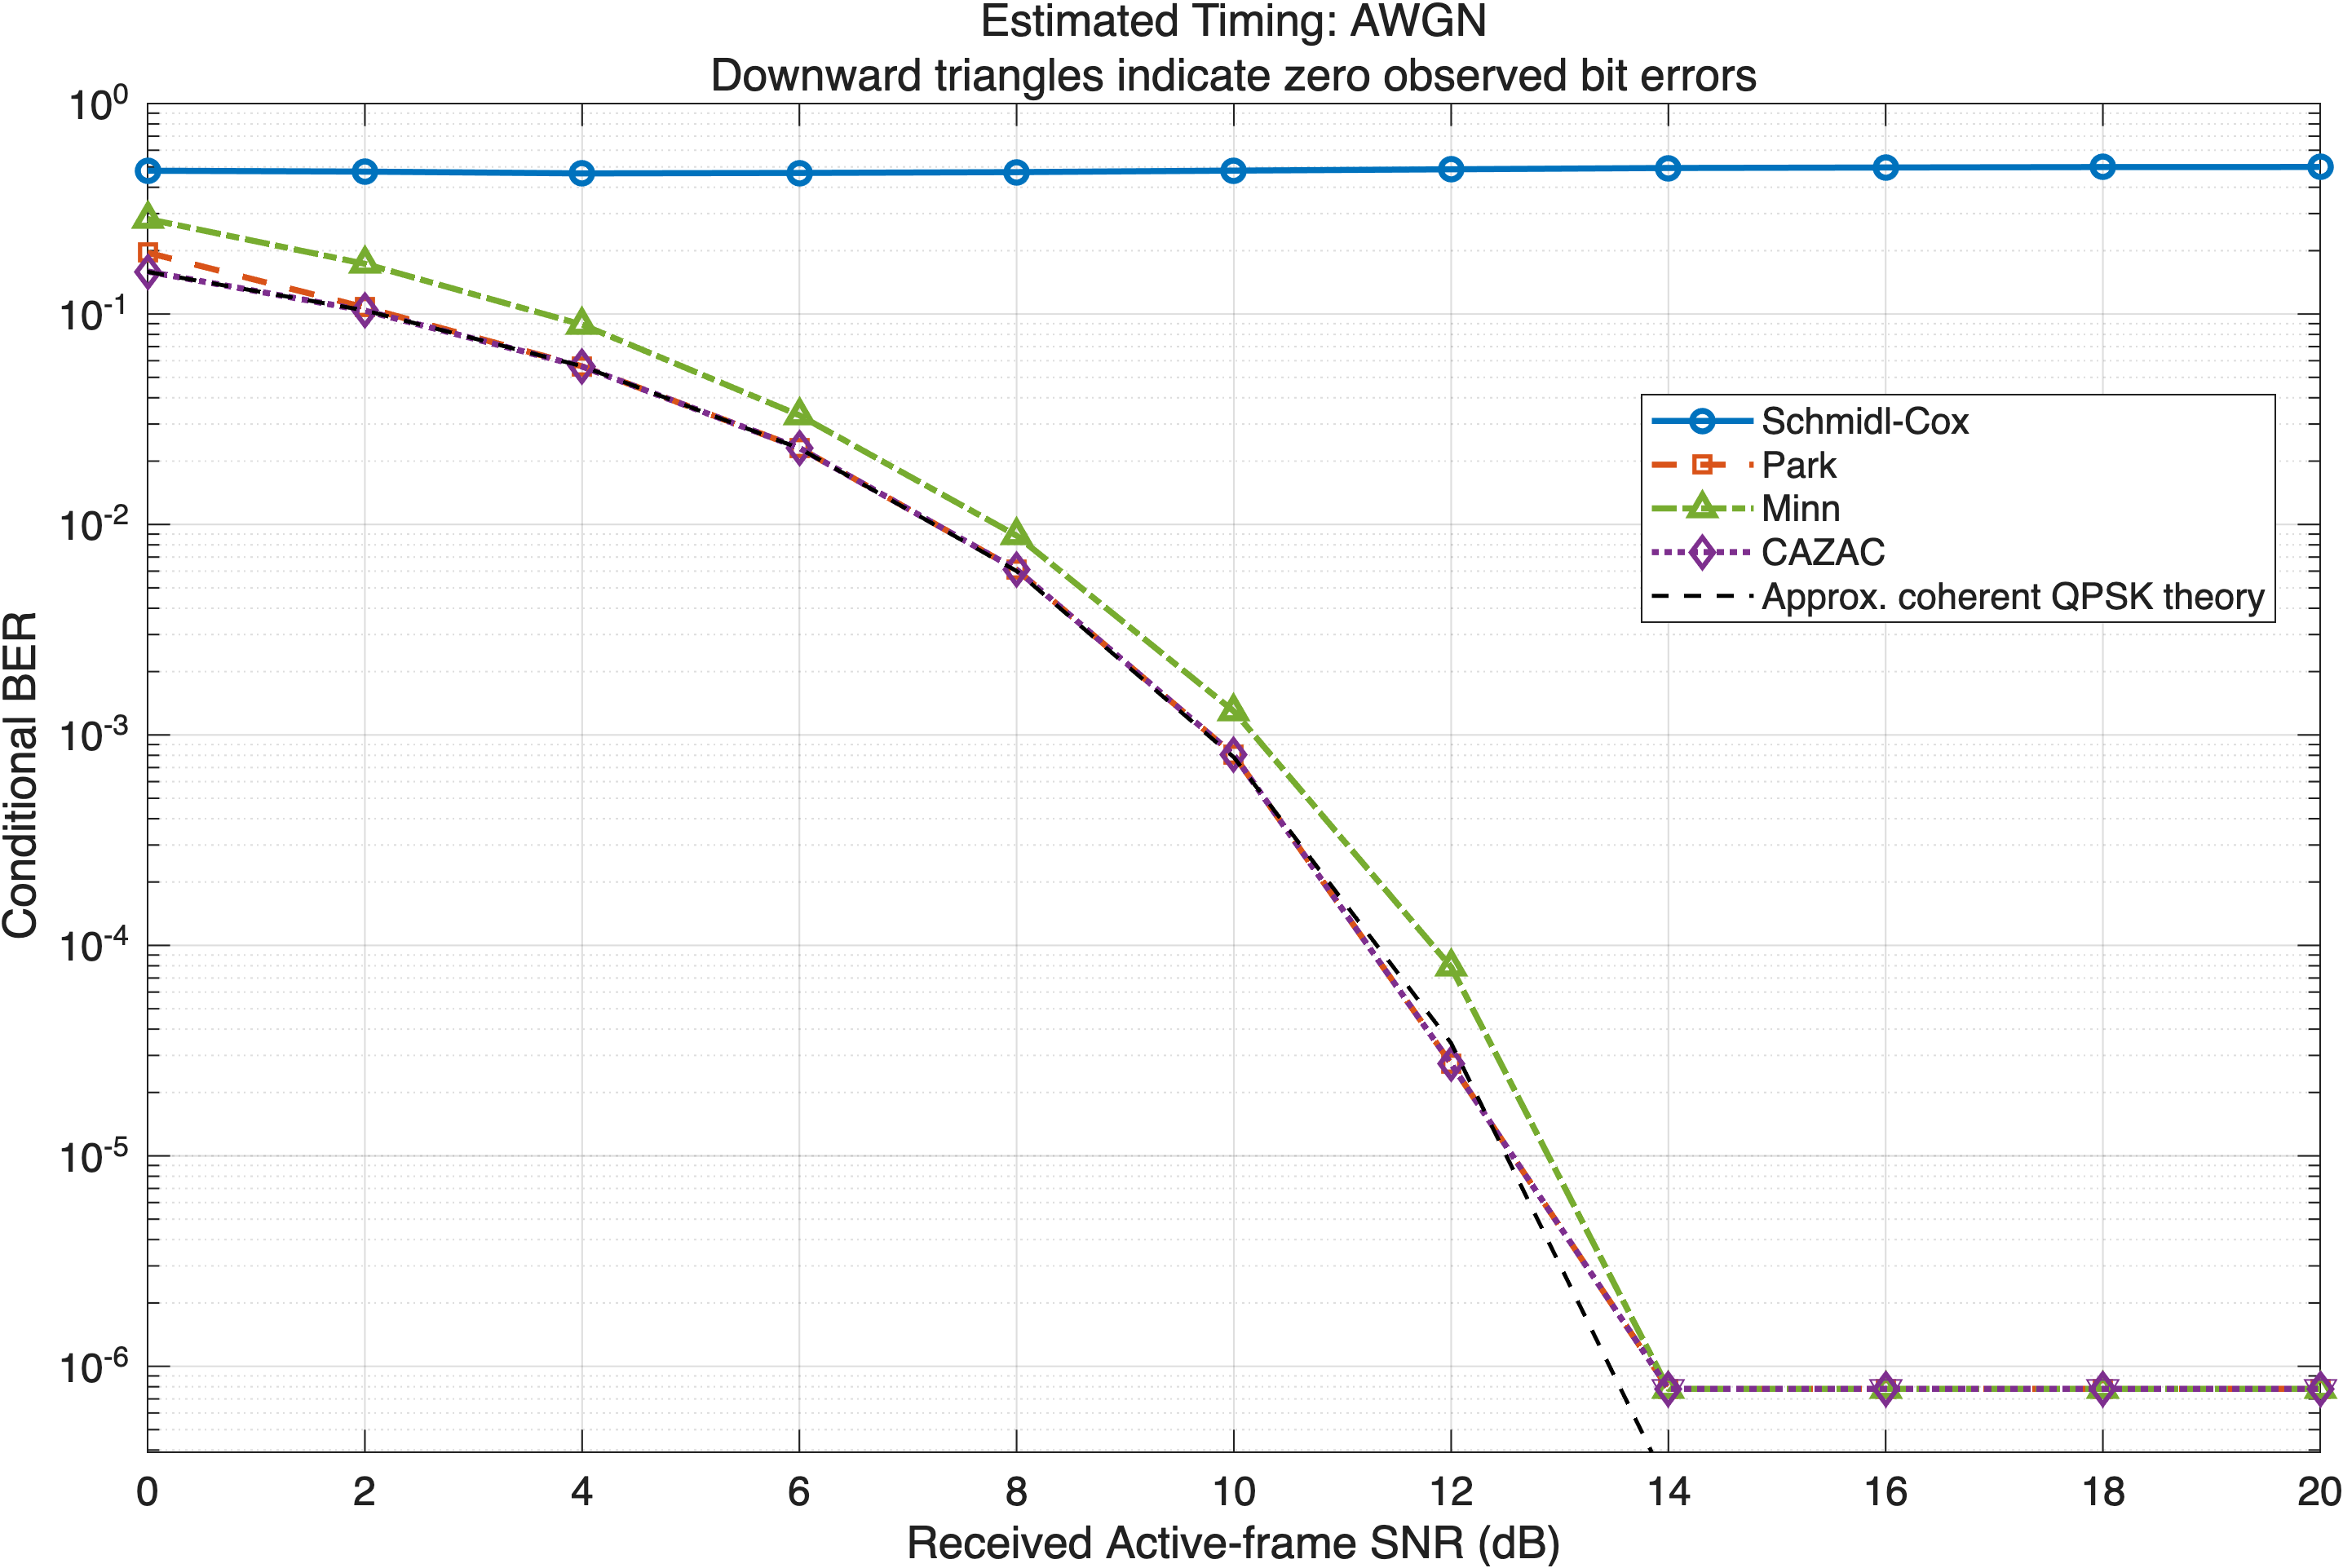
\includegraphics[width=0.90\textwidth,height=0.30\textheight,keepaspectratio]{figures/ch5/exp08_awgn_ber_estimated.png}\par
{\small (a) AWGN}\par\medskip
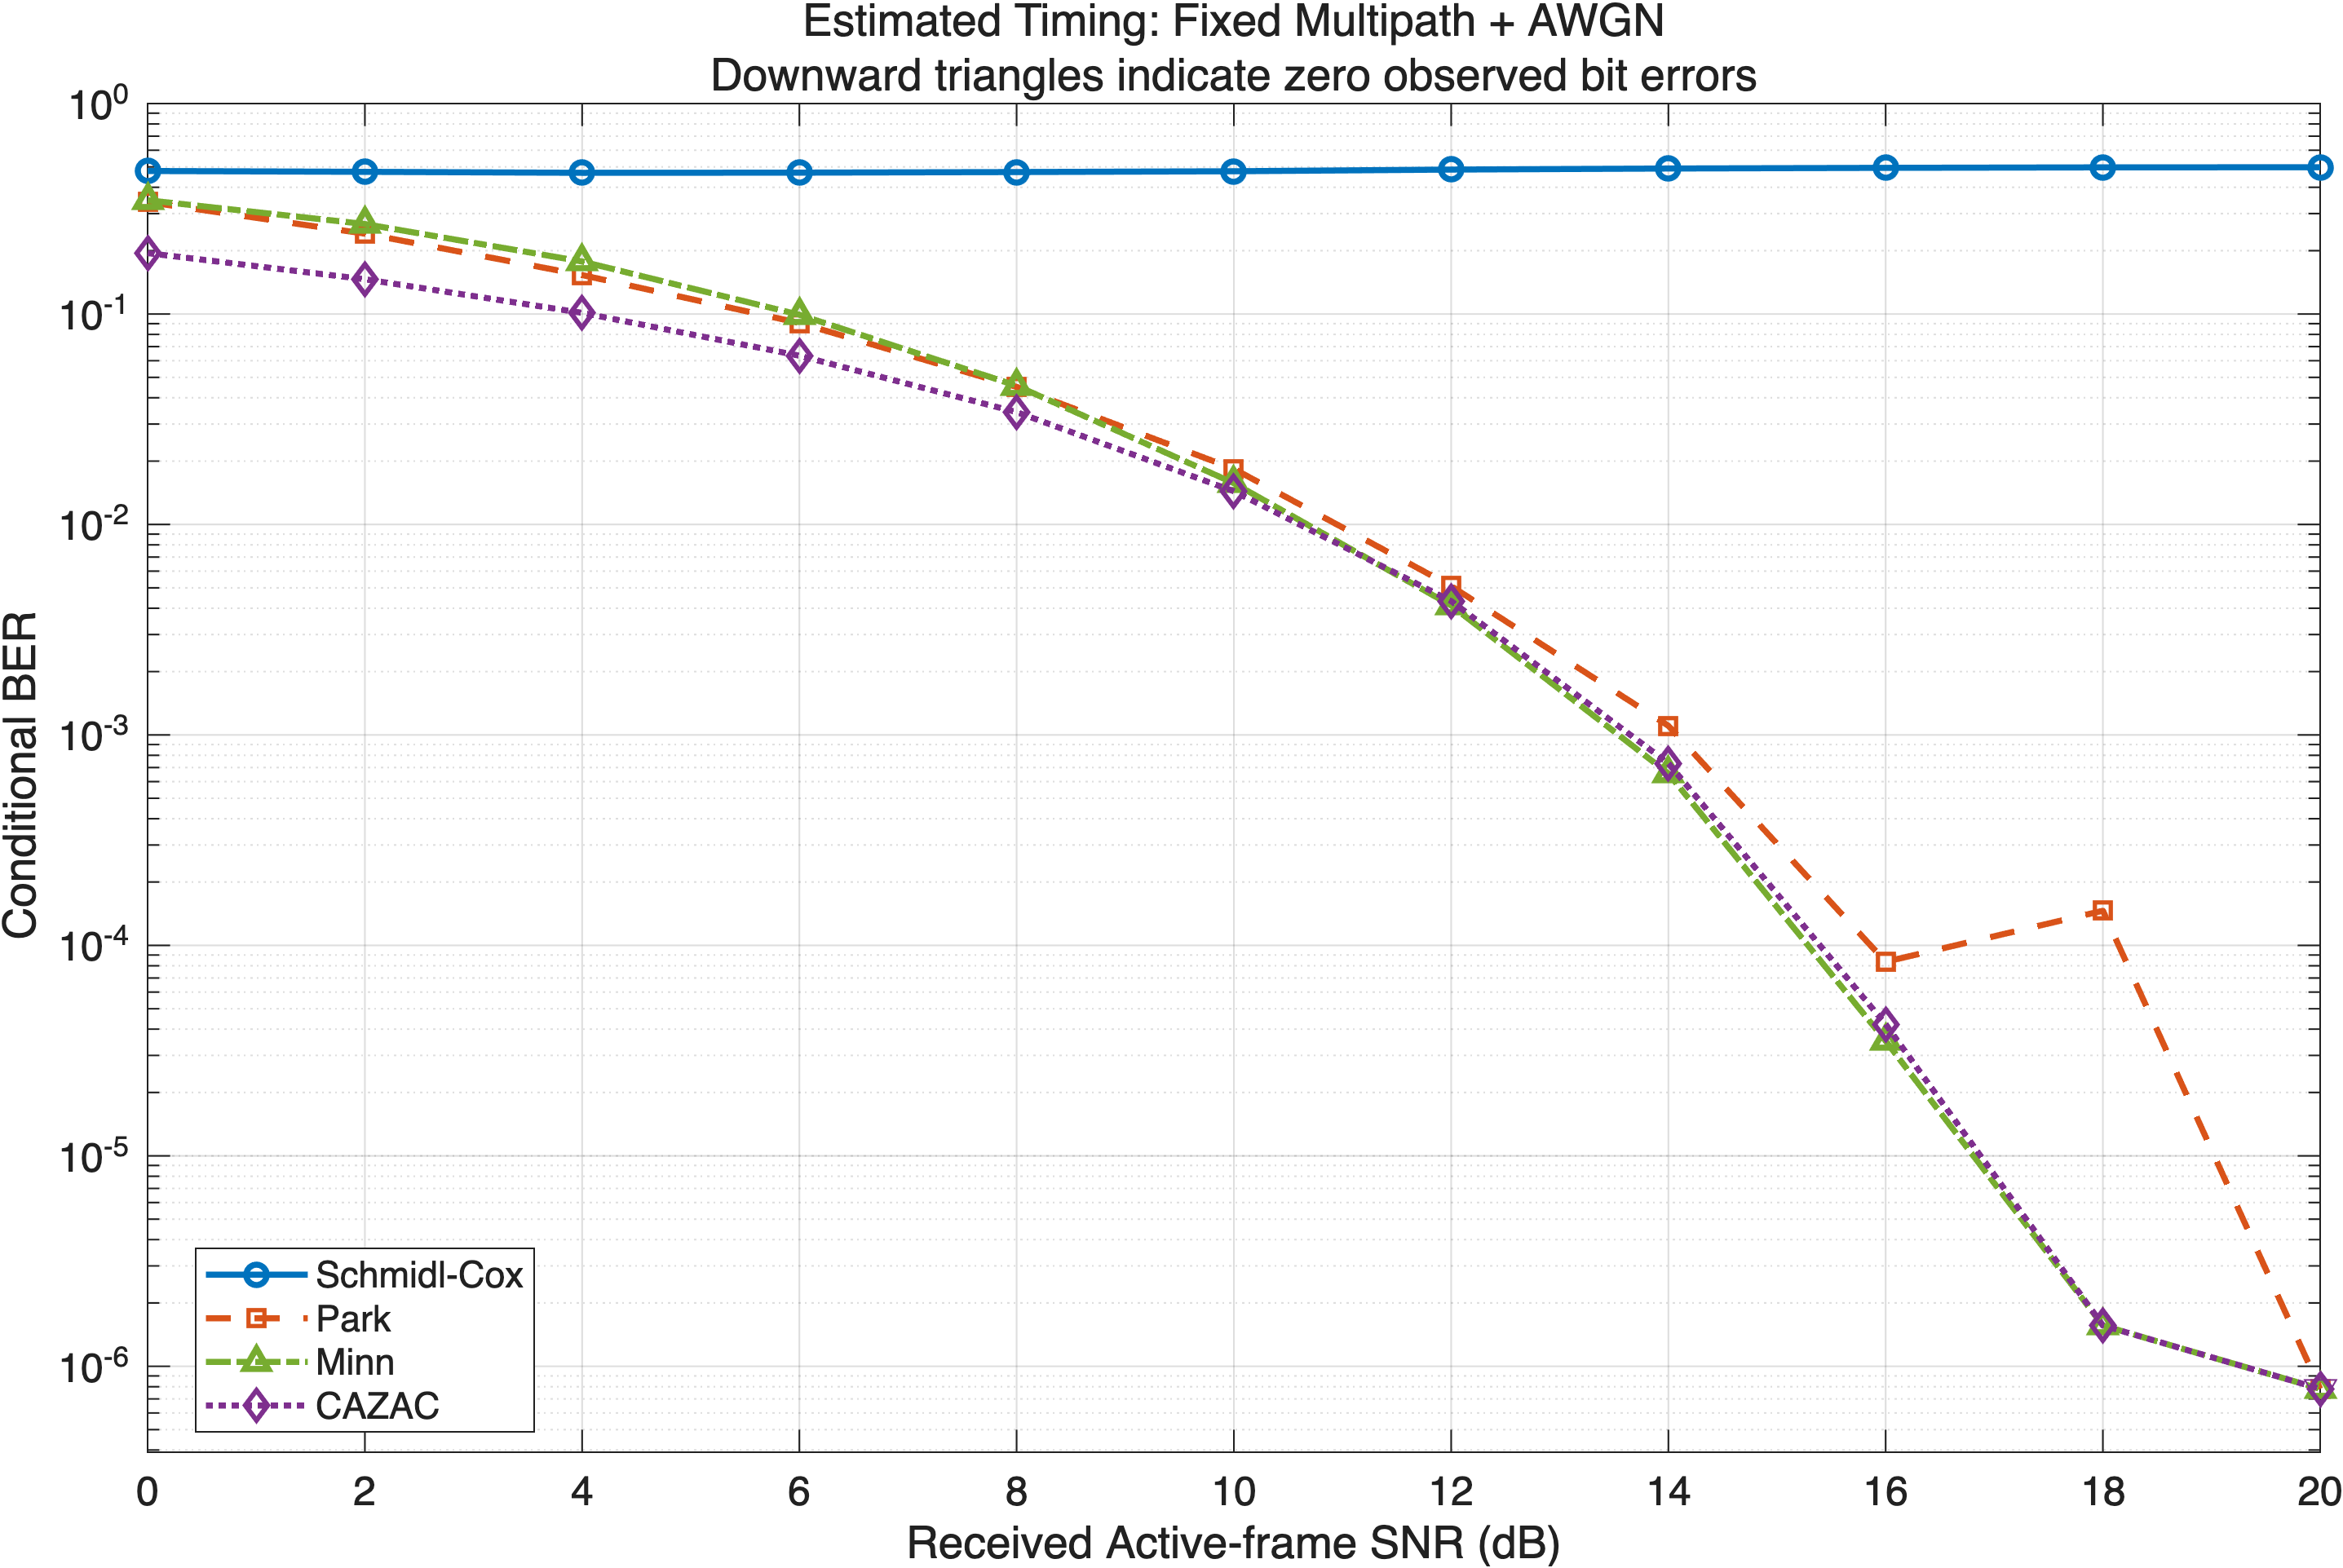
\includegraphics[width=0.90\textwidth,height=0.30\textheight,keepaspectratio]{figures/ch5/exp08_multipath_ber_estimated.png}\par
{\small (b) Fixed multipath with AWGN}
\caption[EXP08: estimated-timing BER.]{EXP08: BER with estimated timing and physical-channel equalization only.}
\label{fig:ch5estimated}
\end{figure}

\begin{table}[!htbp]
\centering\small
\caption[EXP08: bit-error counts in AWGN.]{EXP08: bit-error counts in AWGN. Each entry is based on 1,280,000 decoded bits.}
\label{tab:ch5awgn}
\begin{tabular}{rlrrr}\hline
SNR (dB)&Method&Perfect&Estimated&Oracle\\\hline
0&S\&C&203729&613859&215217\\
 &Park&203729&250434&219592\\
 &Minn&203729&361958&221866\\
 &CAZAC&203729&203729&203729\\\hline
10&S\&C&1029&614662&1296\\
 &Park&1029&1029&1029\\
 &Minn&1029&1657&1199\\
 &CAZAC&1029&1029&1029\\\hline
20&S\&C&0&639428&1\\
 &Park&0&0&0\\
 &Minn&0&0&0\\
 &CAZAC&0&0&0\\\hline
\end{tabular}
\end{table}

\begin{table}[!htbp]
\centering\small
\caption[EXP08: bit-error counts in fixed multipath.]{EXP08: bit-error counts in fixed multipath with AWGN. Each entry is based on 1,280,000 decoded bits.}
\label{tab:ch5mp}
\begin{tabular}{rlrrr}\hline
SNR (dB)&Method&Perfect&Estimated&Oracle\\\hline
0&S\&C&242235&611995&254184\\
 &Park&243741&435782&292434\\
 &Minn&246211&444417&259461\\
 &CAZAC&249122&249240&249121\\\hline
10&S\&C&16293&610322&17375\\
 &Park&16777&23517&16874\\
 &Minn&17511&20102&17548\\
 &CAZAC&18404&18404&18404\\\hline
20&S\&C&0&637574&22\\
 &Park&0&0&0\\
 &Minn&0&0&0\\
 &CAZAC&0&0&0\\\hline
\end{tabular}
\end{table}

\subsection{Performance in AWGN}
At 0 dB, CAZAC returns exact timing for every EXP08 trial and its estimated-timing BER coincides with the perfect reference. Park and Minn have estimated BERs of 0.195652 and 0.282780, respectively. Both exceed the reference of 0.159163 because some windows are displaced. At 10 dB, Park coincides with the reference, while Minn records 1,657 errors compared with the perfect receiver's 1,029. At 20 dB, the three peak-based methods return exact timing and no observed bit errors.

The S\&C result is fundamentally different. Its estimated-timing BER remains close to 0.5 over the SNR grid (0.479577 at 0 dB and 0.499553 at 20 dB). This is not attributable to a failure of the underlying OFDM modulator or FFT: its perfect-timing reference is identical to the other AWGN references. The midpoint decision produces predominantly nonzero early errors, leaving a subcarrier-dependent phase rotation that is not removed by physical-channel equalization.

\subsection{Performance in fixed multipath}
At 0 dB, S\&C has estimated BER 0.478121. The values for Park, Minn and CAZAC are 0.340455, 0.347201 and 0.194719, respectively. Although the Park and Minn curves are close, a comparison of their raw BERs alone conceals the different distributions of timing errors. In EXP08, their CP-safe probabilities at this SNR are 0.5463 and 0.7540, respectively; Minn's larger safe fraction does not imply smaller BER without phase compensation.

By 10 dB the estimated BERs of Park, Minn and CAZAC decrease to 0.018373, 0.015705 and 0.014378, respectively. Their corresponding perfect-timing references are 0.013107, 0.013680 and 0.014378. Thus the remaining synchronization penalties differ even when all three BERs appear similar on a logarithmic plot. At 20 dB all three peak-based designs have no observed bit errors, whereas S\&C has BER 0.498105.

The Park curve in multipath has a small high-SNR irregularity at 18 dB. Examination of its saved frame-level records reveals three nonexact estimates: two errors of $+1$ sample and one of $+10$ samples. These frames contribute 127 and 59 bit errors, respectively, to the uncompensated receiver; one additional error occurs among the 9,997 exactly timed frames. The 187 total errors give BER $1.46094\times10^{-4}$. Oracle compensation reduces the count to one. The subsequent zero-error observation at 20 dB is consistent with rare-event variation; the irregularity is not evidence that increasing SNR systematically worsens the algorithm. These are EXP08 events, distinct from the rare Park errors reported for EXP07.

\section[Oracle Phase Compensation]{Effect of Oracle Phase Compensation}
Figure~\ref{fig:ch5oracle} displays the four algorithms after the oracle compensates the residual phase associated with the true timing error. The compensated receiver still uses the estimated FFT window. It does not move the window back to the correct start. Accordingly, its improvement measures the effect of the supplied phase correction on the existing samples, not a second timing-estimation procedure.

\begin{figure}[!htbp]
\centering
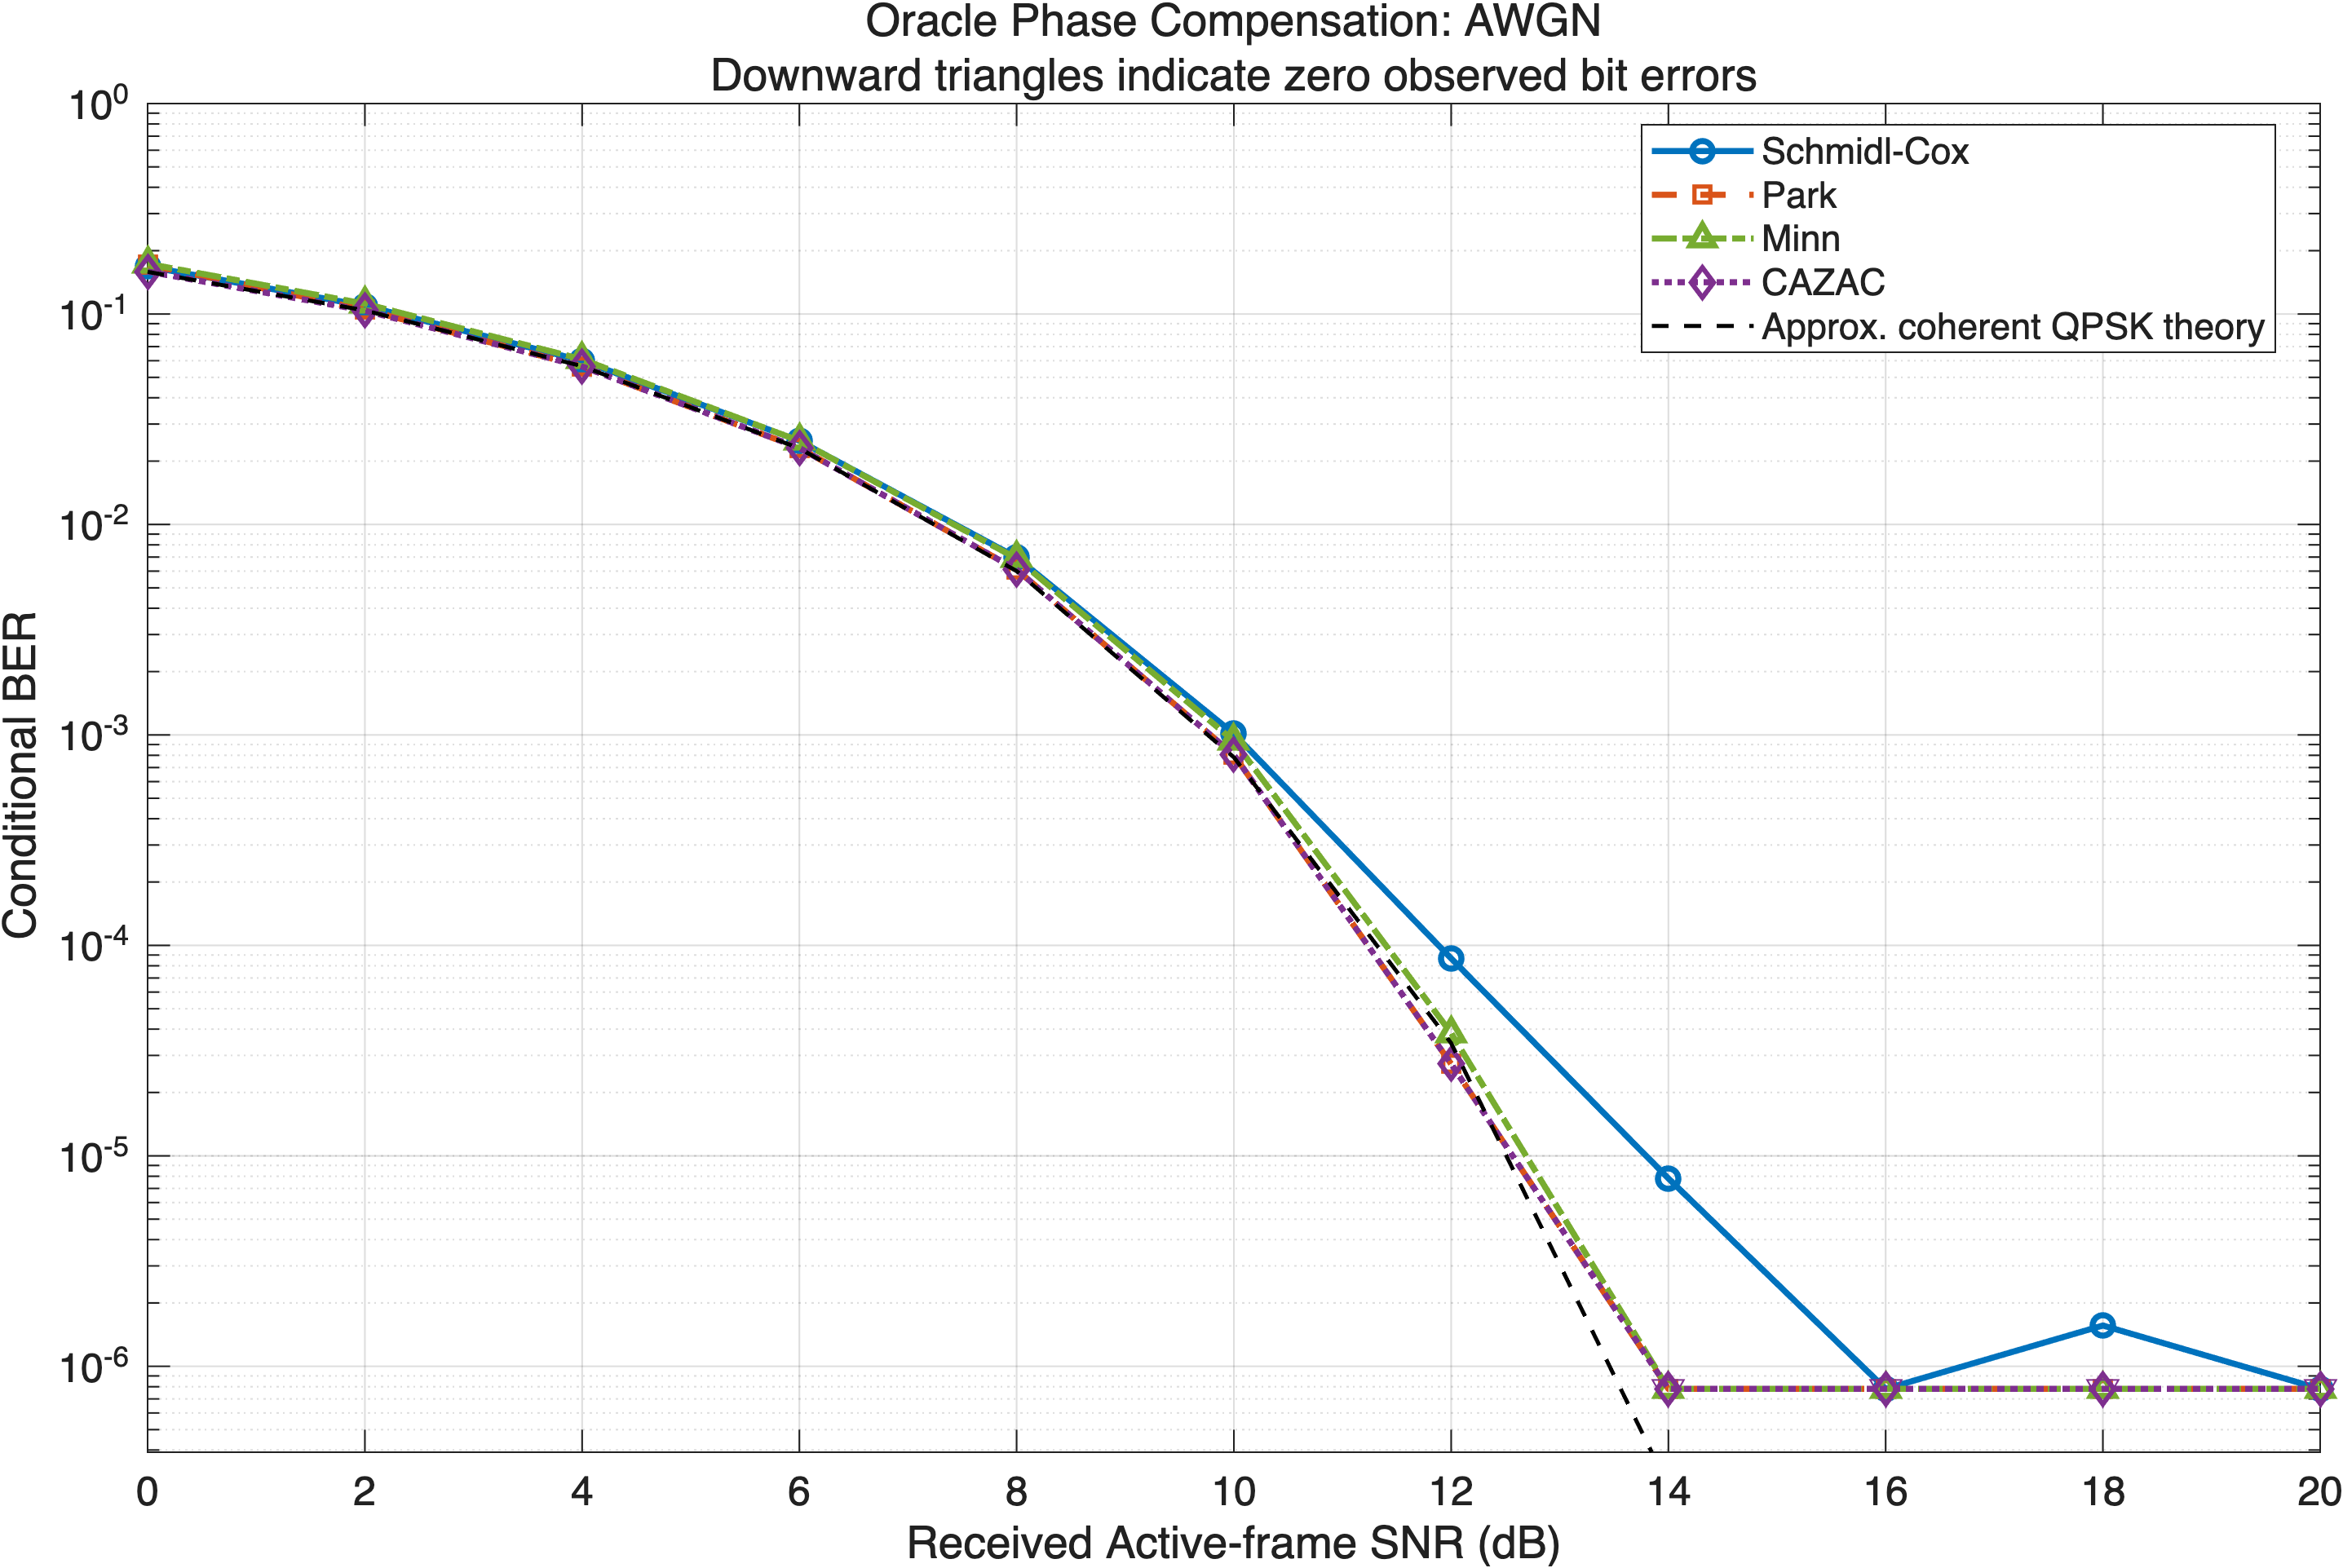
\includegraphics[width=0.90\textwidth,height=0.30\textheight,keepaspectratio]{figures/ch5/exp08_awgn_ber_oracle.png}\par
{\small (a) AWGN}\par\medskip
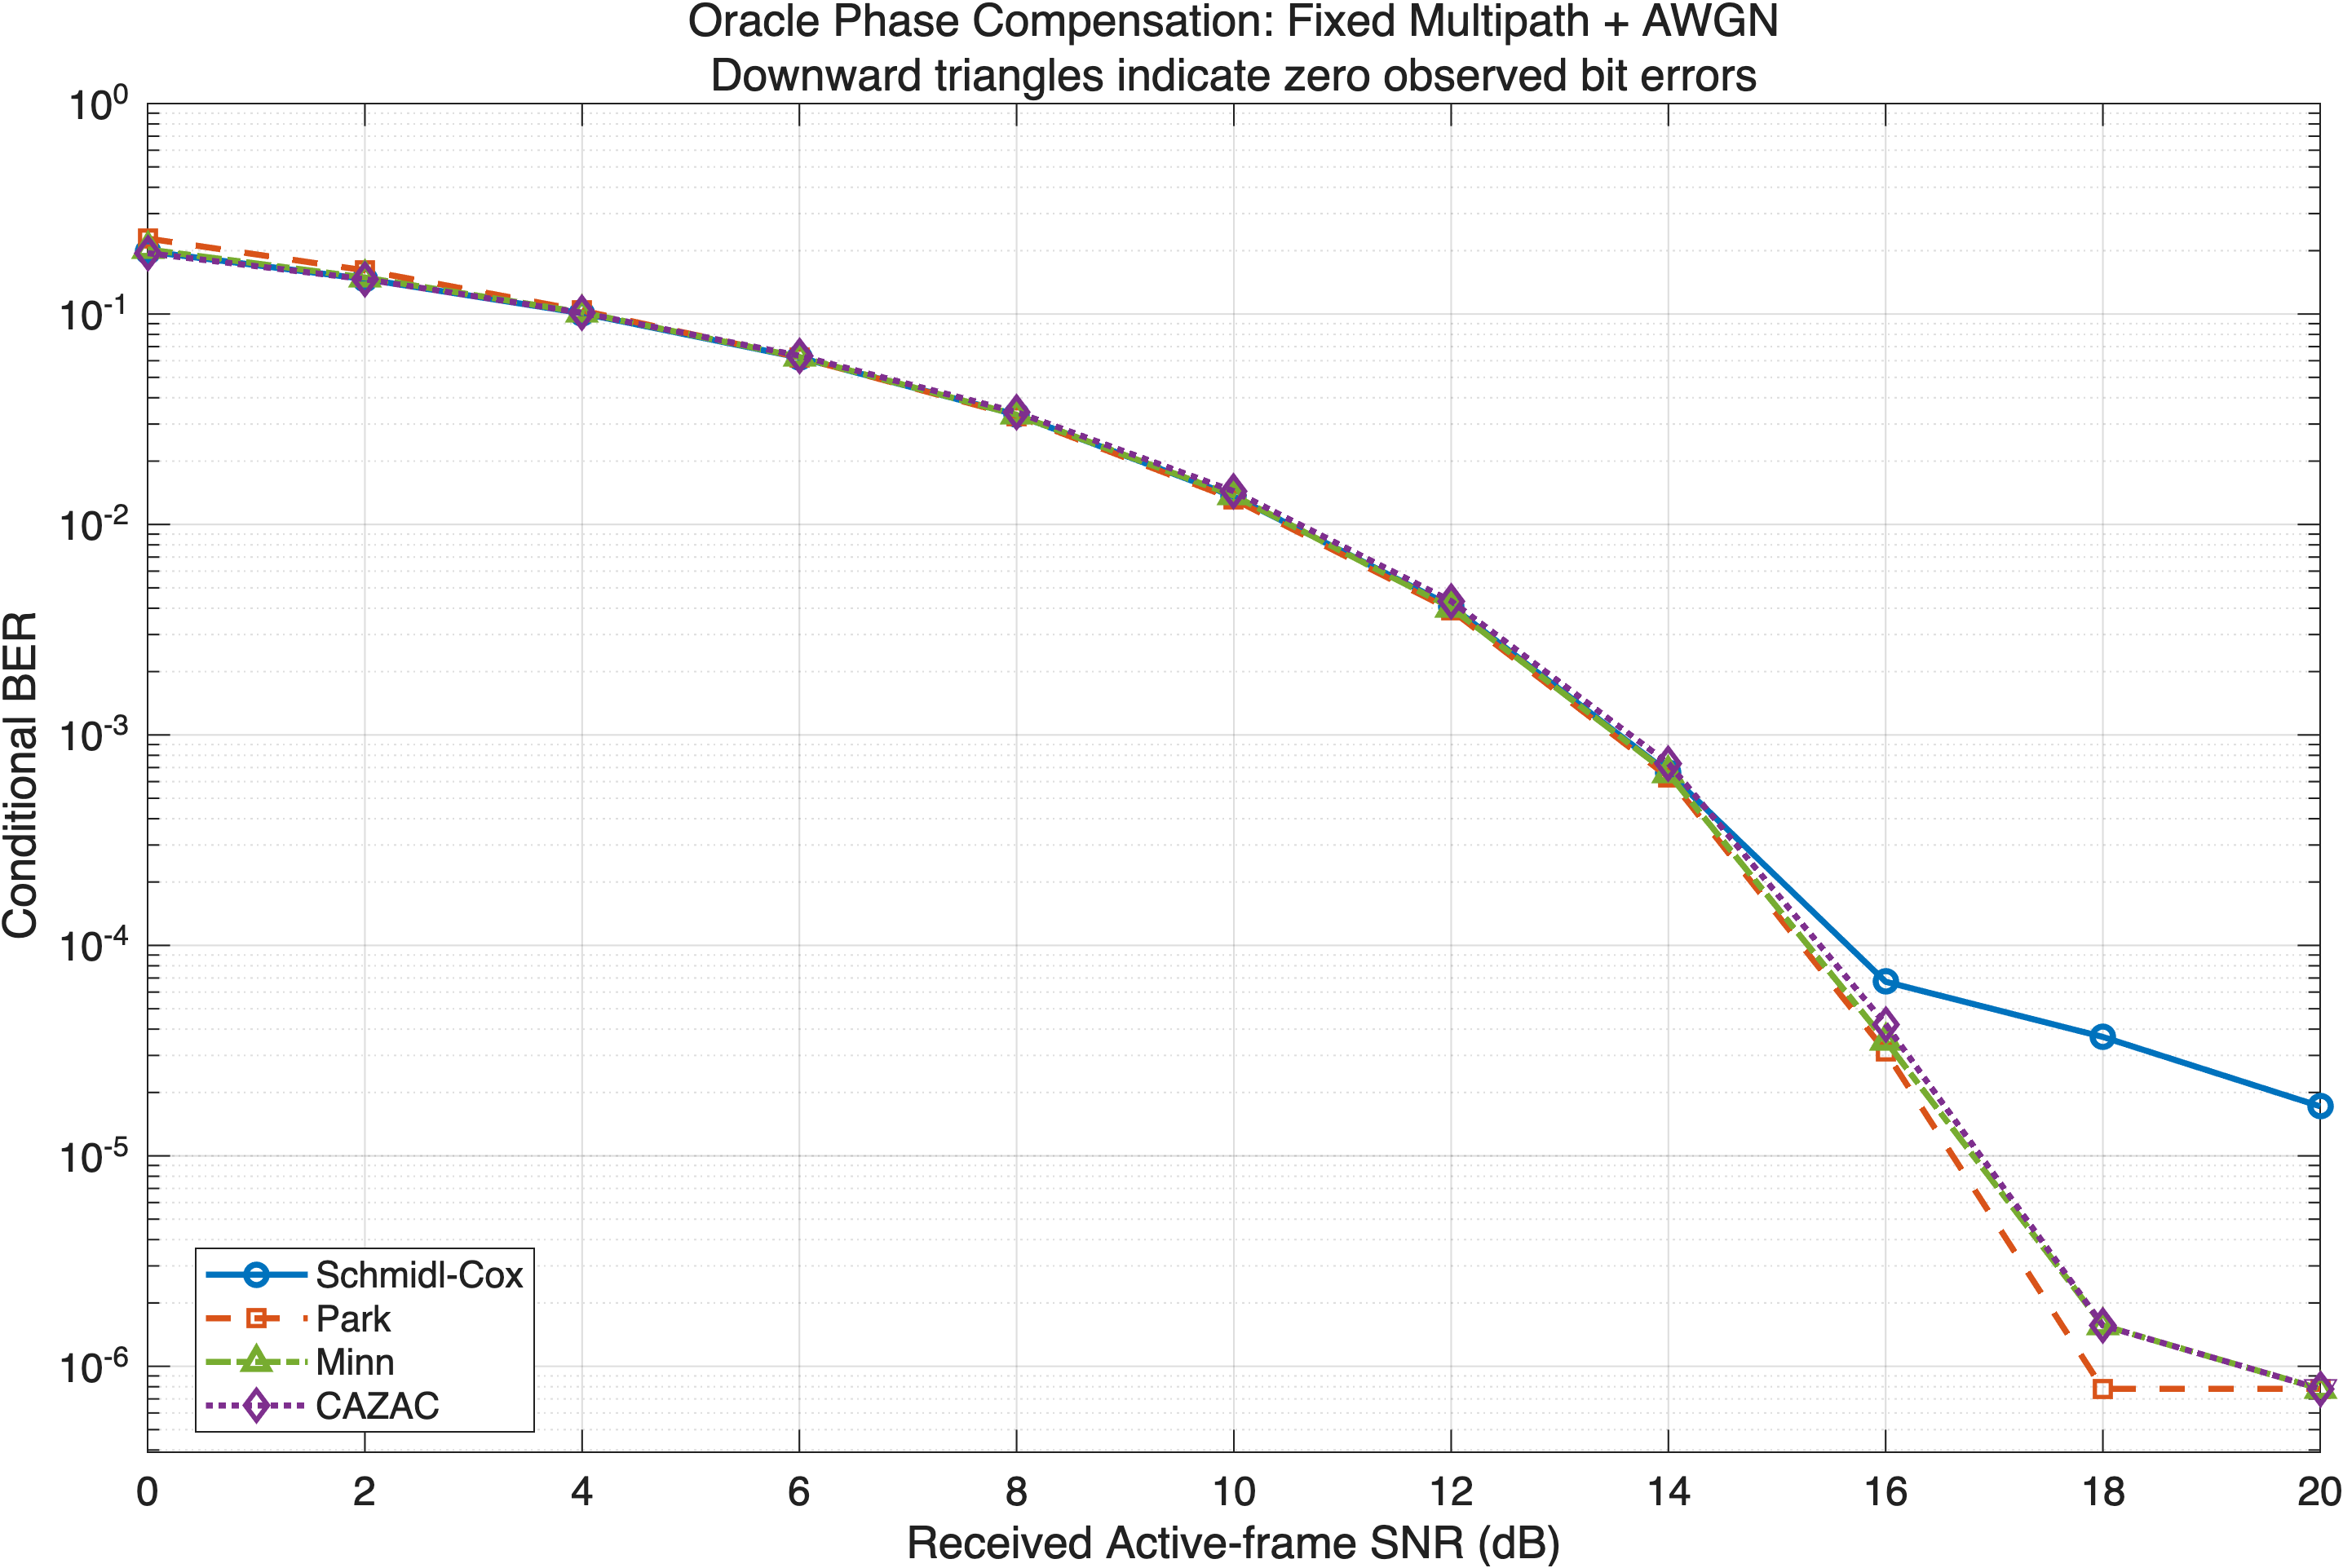
\includegraphics[width=0.90\textwidth,height=0.30\textheight,keepaspectratio]{figures/ch5/exp08_multipath_ber_oracle.png}\par
{\small (b) Fixed multipath with AWGN}
\caption[EXP08: oracle-compensated BER.]{EXP08: BER using the estimated timing window with oracle phase compensation.}
\label{fig:ch5oracle}
\end{figure}

The improvement is most pronounced for S\&C, as illustrated by the direct receiver comparisons in Figure~\ref{fig:ch5sc}. At 10 dB AWGN, its 614,662 uncompensated bit errors decrease to 1,296 with compensation, compared with 1,029 for perfect timing. At 20 dB AWGN, its count decreases from 639,428 to one, while the perfect receiver records zero. In multipath at 20 dB, compensation reduces 637,574 errors to 22. These changes strongly support the phase-rotation mechanism developed in Chapter 2 and verified in EXP02.

\begin{figure}[!htbp]
\centering
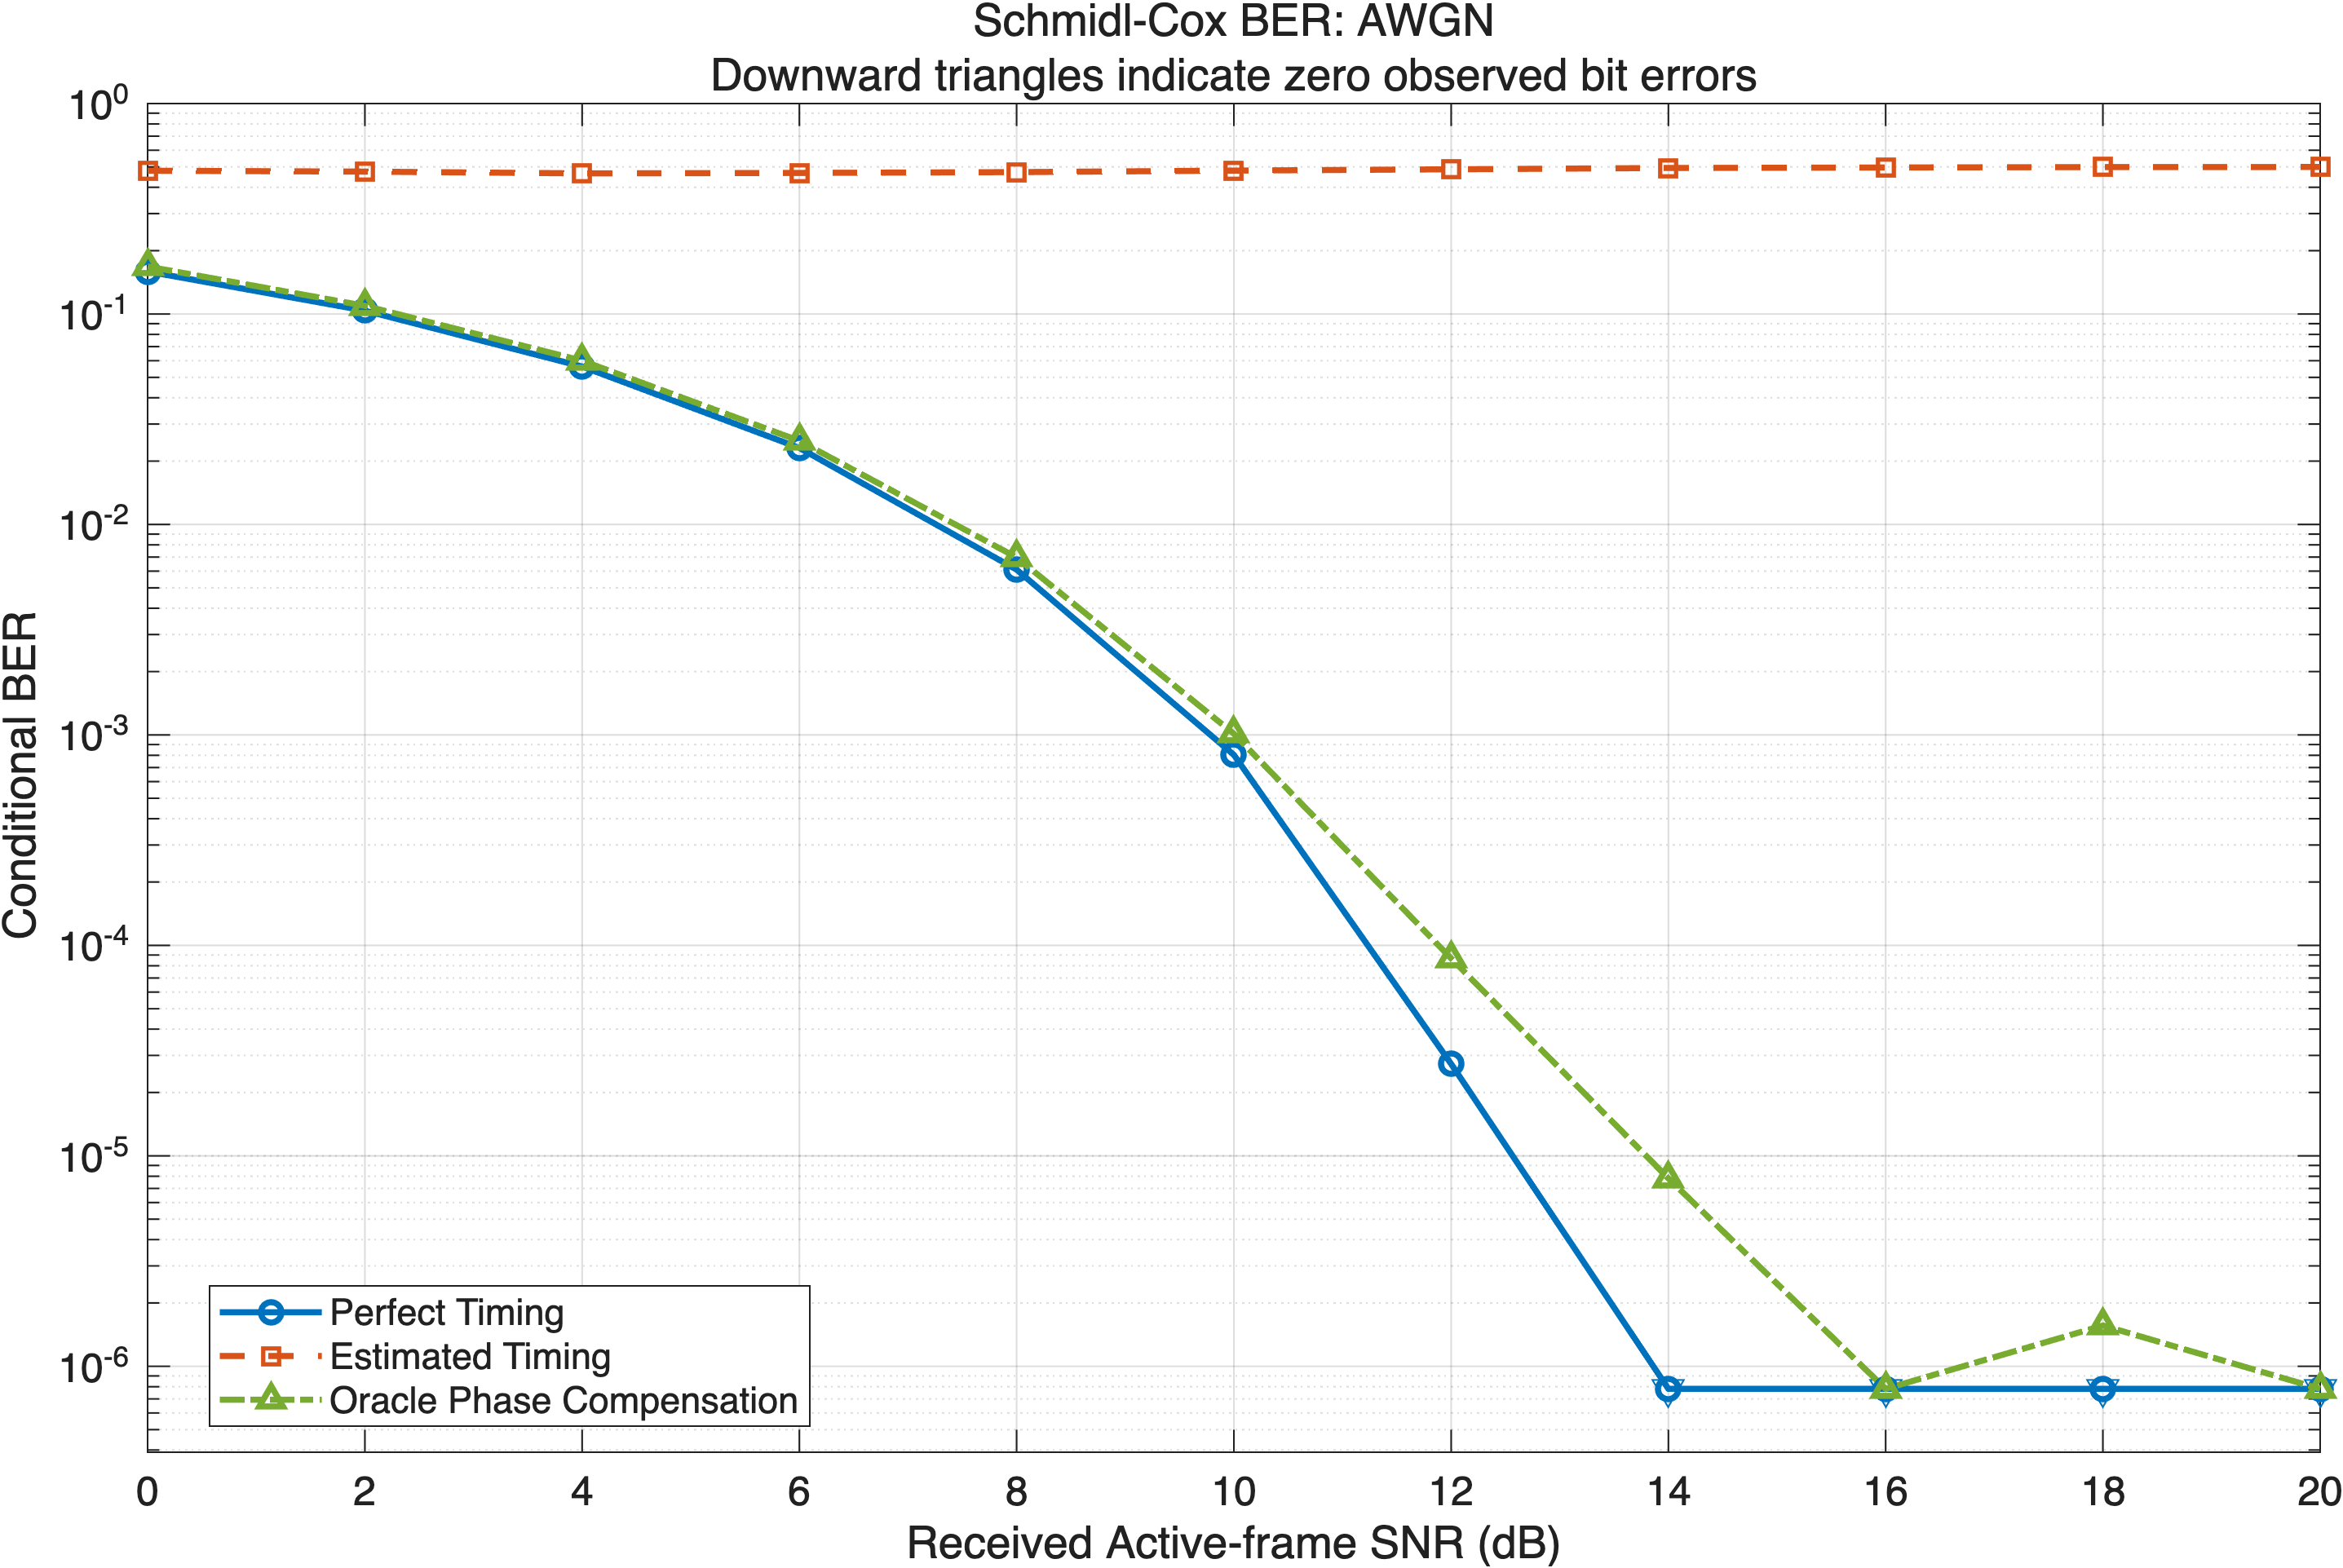
\includegraphics[width=0.90\textwidth,height=0.30\textheight,keepaspectratio]{figures/ch5/exp08_awgn_sc_receiver_comparison.png}\par
{\small (a) AWGN}\par\medskip
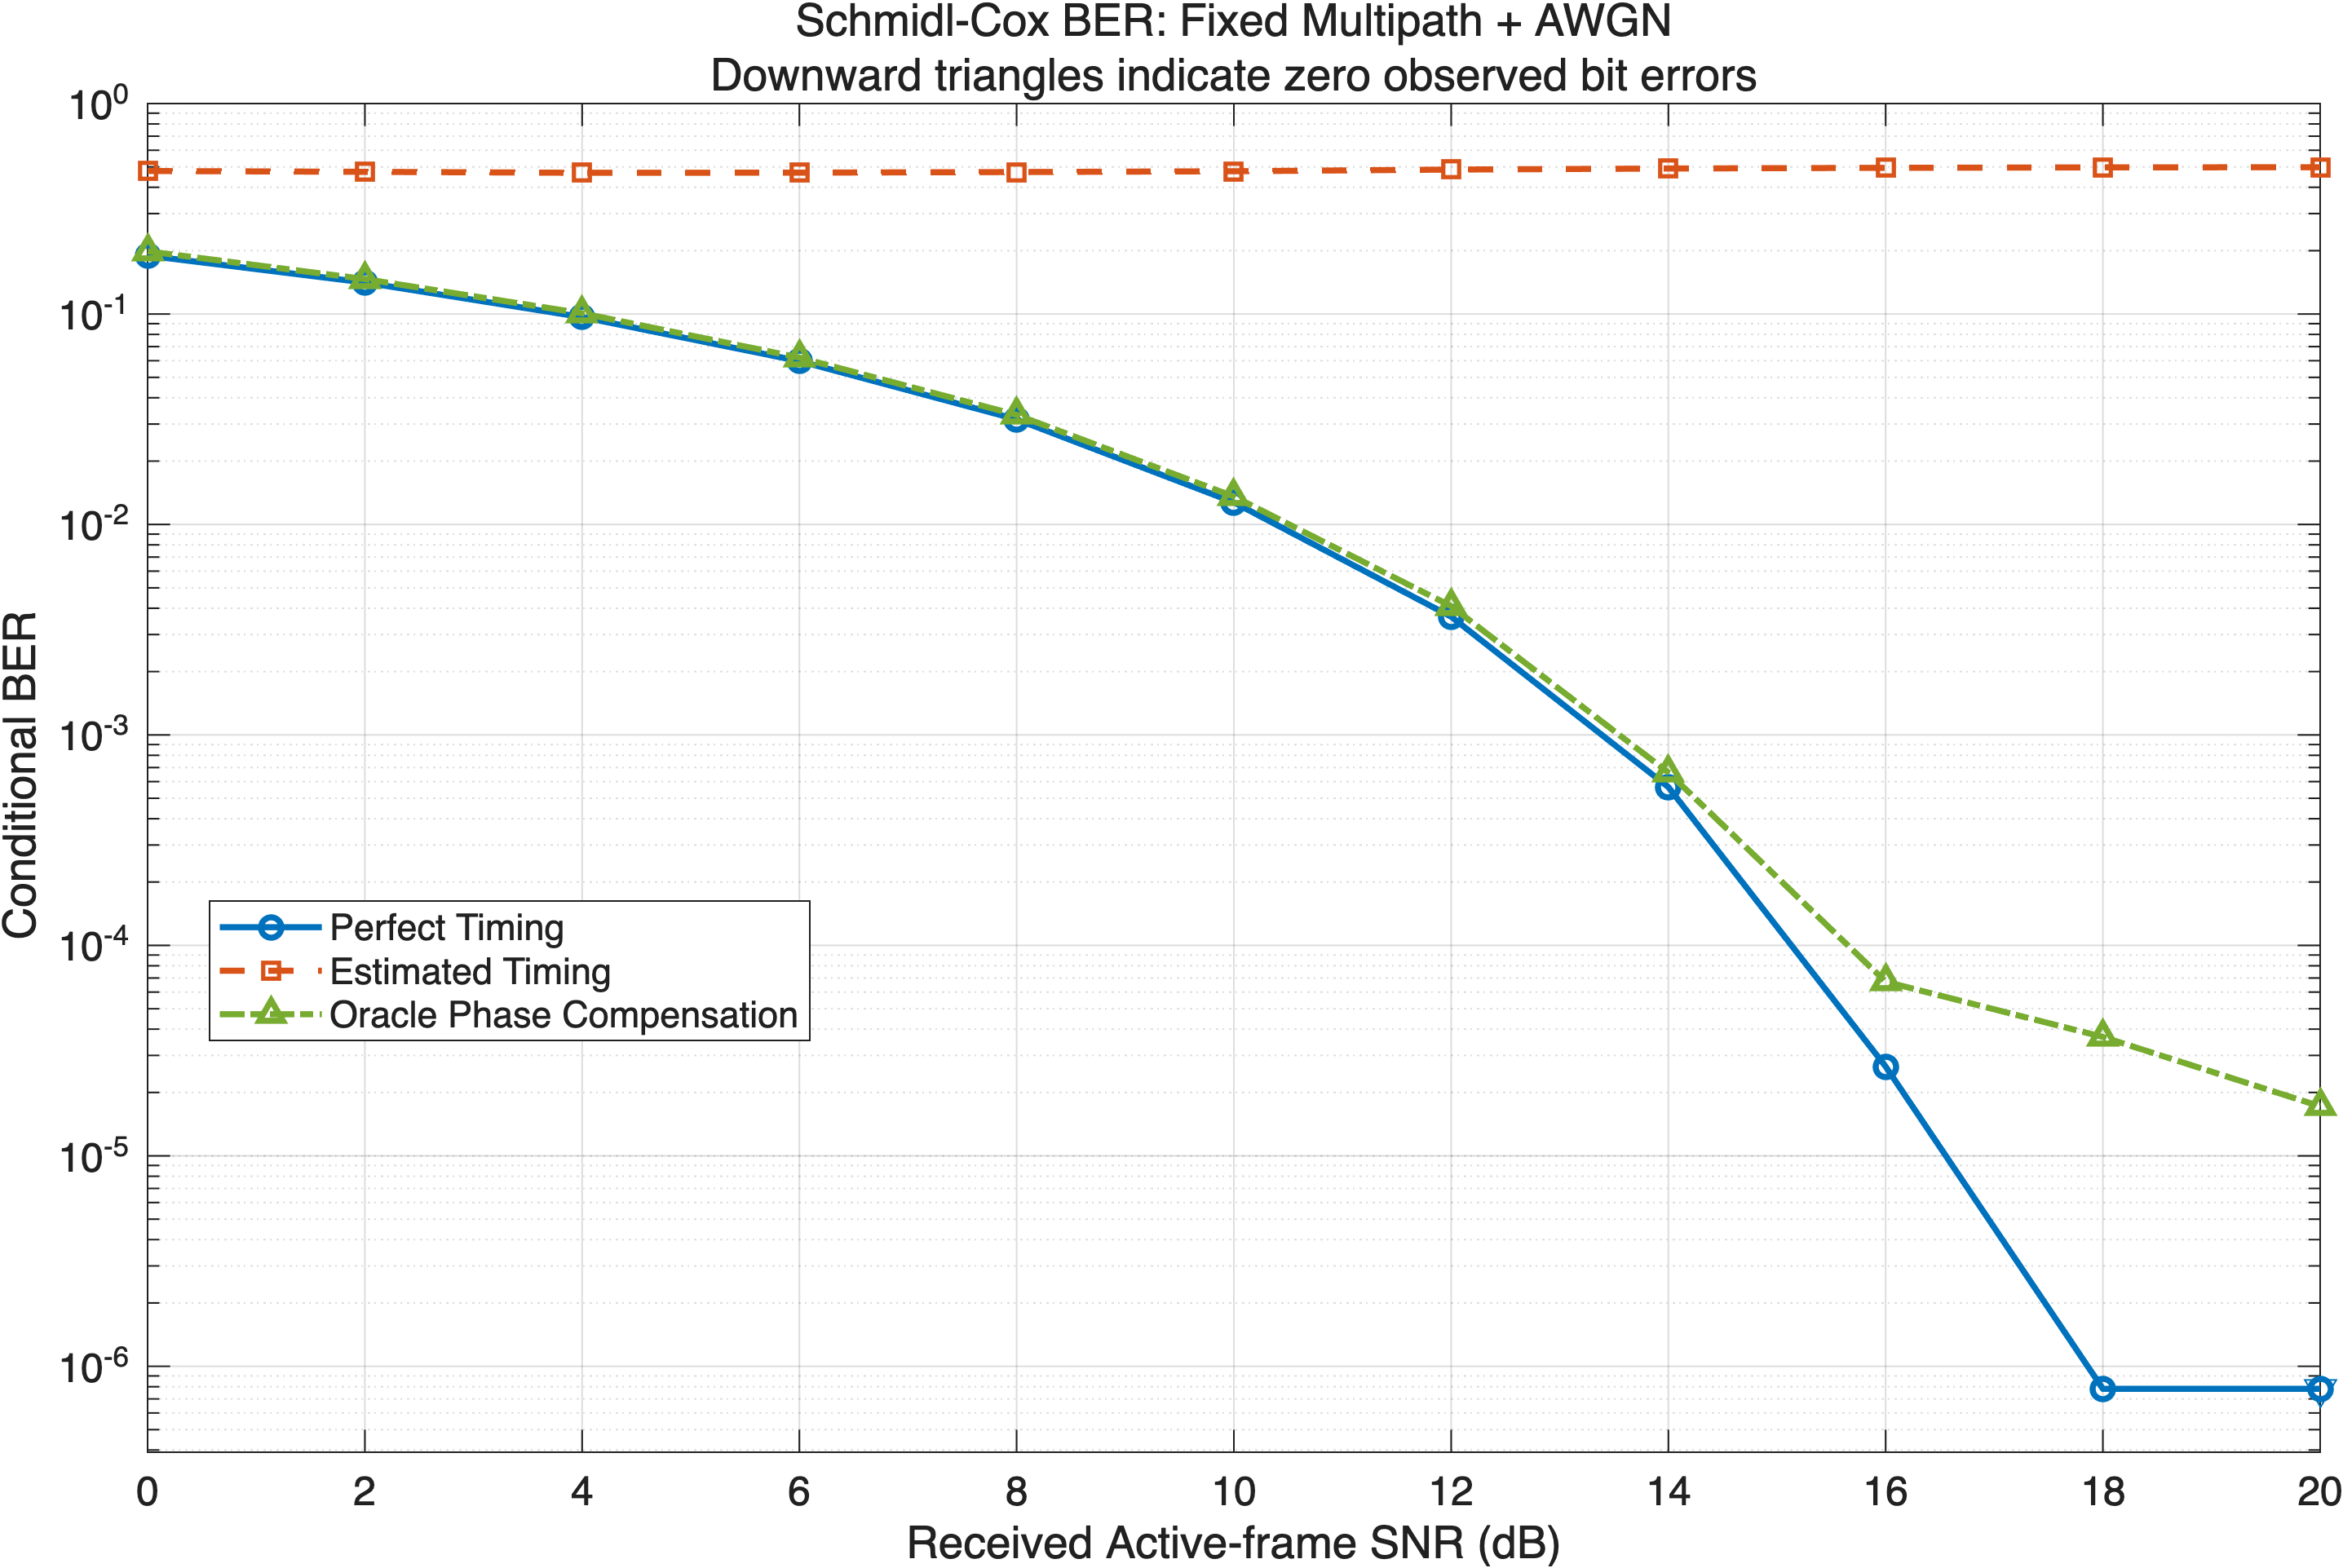
\includegraphics[width=0.90\textwidth,height=0.30\textheight,keepaspectratio]{figures/ch5/exp08_multipath_sc_receiver_comparison.png}\par
{\small (b) Fixed multipath with AWGN}
\caption[EXP08: S\&C receiver comparison.]{EXP08: comparison of perfect, estimated and oracle receiver cases for S\&C.}
\label{fig:ch5sc}
\end{figure}

The peak-based estimators also benefit when nonexact estimates occur. At 0 dB multipath, Park's oracle BER is 0.228464 and Minn's is 0.202704, compared with their respective perfect references of 0.190423 and 0.192352. These differences are consistent with their different error distributions and rates of unsafe-window selection. CAZAC has only three nonexact timing observations across EXP08, all $+1$ sample in 0 dB multipath. For this condition its compensated count (249,121) is one less than the perfect reference (249,122). Small differences of either sign are possible because displaced windows observe different noise samples and can experience different distortion. Perfect timing provides a reference, not a deterministic lower bound on the bit-error count of each realization.

\section[CP-Safe Timing and BER]{Relationship between CP-Safe Timing and BER}
\label{sec:ch5safe}
The aggregate BER can be expressed as a mixture over the estimated-window timing categories. Let $S$ denote a CP-safe timing estimate, and let $U$ be its complement. Since all frames are valid and carry the same number of bits, for a fixed receiver case the empirical decomposition is
\begin{equation}
\widehat{\mathrm{BER}}=\hat p_S\widehat{\mathrm{BER}}_S
 +(1-\hat p_S)\widehat{\mathrm{BER}}_U,
\label{eq:ch5mixture}
\end{equation}
where $\hat p_S$ is the fraction of safe estimates in the same EXP08 condition. A category with no observations has an undefined conditional BER and contributes zero to the total error count. This identity does not require independence between timing error and bit errors.

\begin{table}[!htbp]
\centering\small
\caption[EXP08: S\&C errors by timing category at 20 dB.]{EXP08: S\&C bit-error counts by timing category at 20 dB. Every frame contains 128 decoded bits.}
\label{tab:ch5safe}
\begin{tabular}{llrrr}\hline
Channel&Category&Frames&Estimated&Oracle\\\hline
AWGN&Safe&9981&638209&0\\
&Unsafe&19&1219&1\\\hline
Multipath&Safe&9905&631491&0\\
&Unsafe&95&6083&22\\\hline
\end{tabular}
\end{table}

Table~\ref{tab:ch5safe} shows that 99.81\% of the S\&C estimates in AWGN and 99.05\% in multipath are CP-safe at 20 dB. Nevertheless, the uncompensated BER restricted to safe frames is 0.499550 in AWGN and 0.498084 in multipath. After oracle compensation, there are no observed bit errors among safe frames in either channel. All remaining oracle bit errors occur in the unsafe category. The 19 unsafe AWGN frames produce one error, and the 95 unsafe multipath frames produce 22, giving conditional unsafe BERs of $4.11\times10^{-4}$ and $1.81\times10^{-3}$, respectively. Thus a small fraction of frames accounts for the entire residual error count in these particular high-SNR conditions.

The circular-convolution result in Section~2.3 explains this observation. With physical-channel equalization only and a safe integer offset $e$, the noise-free subcarrier symbol is proportional to
\begin{equation}
X[k]\exp(j2\pi ke/N).
\end{equation}
For the typical nonzero S\&C errors, the phase progression spans the QPSK decision regions. For example, at $e=-7$ the phase sequence visits all 64 equally spaced angles because 7 and 64 are relatively prime. Subcarriers separated by 32 indices then have opposite phase factors. For equiprobable Gray-coded QPSK, decisions related by a rotation of $\pi$ have complementary bit labels; away from decision-boundary ties, the paired bit-error counts average one error per two bits. Symmetric noise also preserves this complementarity in expectation under equal subcarrier noise conditions. This illustrates why the uncompensated aggregate BER can approach 0.5 even when the FFT window is structurally safe. It is not a claim that every nonzero offset, modulation scheme or finite trial must have BER exactly 0.5.

The oracle removes the deterministic phase progression but does not undo ISI, ICI or missing samples outside the safe interval. Conversely, an unsafe estimate need not produce a bit error in every frame, especially for a small displacement at high SNR. Hence exact probability, CP-safe probability and BER should be reported together rather than substituted for one another.

\section[Paired Statistical Interpretation]{Paired Statistical Interpretation}
A comparison of receiver cases on the same frame can quantify the average benefit of oracle compensation without treating the 128 bits within a frame as independent Bernoulli observations. Let $B_{i,E}$ and $B_{i,O}$ be the estimated and oracle bit-error counts for frame $i$, and define the paired frame-level difference
\begin{equation}
\Delta_i=\frac{B_{i,E}-B_{i,O}}{128}.
\end{equation}
Because all frames are valid, the sample mean $\bar\Delta$ equals the difference between the two aggregate BERs. Under independent frame trials within a fixed condition, its estimated Monte Carlo standard error is
\begin{equation}
\widehat{\mathrm{SE}}(\bar\Delta)=
\sqrt{\frac{1}{K(K-1)}\sum_{i=1}^{K}(\Delta_i-\bar\Delta)^2},
\qquad K=10{,}000.
\end{equation}
This estimate accounts for the pairing and allows arbitrary dependence among the bit decisions within each frame. It quantifies simulation uncertainty for the specified condition, not variability across untested channels or hardware.

\begin{table}[!htbp]
\centering\small
\caption[EXP08: paired BER reductions.]{EXP08: mean paired reduction in BER (estimated minus oracle) and its frame-level Monte Carlo standard error.}
\label{tab:ch5paired}
\begin{tabular}{llrr}\hline
Condition&Method&$\bar\Delta$&$\widehat{\mathrm{SE}}$\\\hline
AWGN, 20 dB&S\&C&0.499552&0.000211\\
MP, 20 dB&S\&C&0.498088&0.000270\\
MP, 0 dB&Park&0.111991&0.001287\\
MP, 0 dB&Minn&0.144497&0.001397\\\hline
\end{tabular}
\end{table}

Table~\ref{tab:ch5paired} reports selected conditions calculated directly from the frozen EXP08 bit-error arrays. The high-SNR S\&C reductions of approximately 0.5 are much larger than the corresponding Monte Carlo standard errors. At 0 dB multipath, Minn also shows a substantial reduction despite its slightly higher uncompensated BER than Park. These values describe the benefit of providing the true timing error for phase compensation, not the achievable benefit of an implemented practical phase estimator.

The BER resolution of $1/1{,}280{,}000$ describes the smallest nonzero recorded fraction. It does not by itself quantify statistical uncertainty, because bit errors can cluster within a mistimed frame. In particular, a binomial interval treating all 1,280,000 bits as independent would not be justified by the experimental design. A zero-error condition can instead be interpreted at frame level using the independent-frame assumption, with the same per-condition binomial bound discussed in Section~4.7 for the probability that a frame has any bit error. No simultaneous significance claim over the full grid is made here.

\section[Computational Complexity]{Computational Complexity}
\label{sec:ch5complexity}
A performance comparison is incomplete without considering the processing required to obtain timing estimates. The following analysis counts terms in the direct correlation sums implemented by the frozen MATLAB functions; it is not a measurement of execution time or hardware resource use. Let $C$ denote the number of evaluated candidate positions. For a common decision interval of $C=93$, the repeated-half and mirror correlations each contain $N/2=32$ complex products per candidate. The Minn-type metric computes three adjacent-block correlations of length $N/4=16$, giving 48 products. The CAZAC matched filter uses the entire CP-inclusive preamble and therefore evaluates $N+G=80$ products.

\begin{table}[!htbp]
\centering\small
\caption[Direct correlation workload.]{Direct correlation-product counts. The full-buffer counts describe the metric loops in the frozen implementation; the common-range counts are hypothetical direct evaluations on the 93 decision candidates only.}
\label{tab:ch5complexity}
\begin{tabular}{lrrrr}\hline
Method&Per cand.&93 cand.&Full cand.&Full products\\\hline
S\&C&32&2976&243&7776\\
Park&32&2976&243&7776\\
Minn&48&4464&243&11664\\
CAZAC&80&7440&227&18160\\\hline
\end{tabular}
\end{table}

The actual code computes the metric over every complete window of the 306-sample buffer before restricting its decision range. A 64-sample window therefore yields $306-64+1=243$ candidates, whereas an 80-sample window yields $306-80+1=227$. The resulting direct product counts are shown in Table~\ref{tab:ch5complexity}. The common-range column provides a consistent measure of the principal correlation workload but is not the number of products executed by the frozen code.

The counts exclude the energy calculations, normalization, candidate filtering and decisions. In the full-buffer loops, S\&C calculates 32 received-sample magnitude-squared terms per candidate for the right-half energy. Park calculates 32 such terms for its diagnostic right-half energy, performs a global maximum and normalization, and separately recomputes both half energies (64 terms per candidate) for all 93 positions in the search interval. Minn calculates 64 received-sample energy terms per candidate, and CAZAC calculates 80, plus the 80 template energy terms once per metric call. These correspond to 7,776, 7,776 plus 5,952, 15,552 and 18,160 plus 80 energy terms, respectively. S\&C additionally searches the contiguous threshold region around the selected maximum, while the other estimators select a peak among eligible candidates. Minn's sign weighting and CAZAC's deterministic template generation introduce further operations not included in the complex-product counts.

For direct window-by-window evaluation, the leading correlation complexity is $O(CN)$ for S\&C, Park and Minn, and $O(C(N+G))$ for CAZAC. With a fixed ratio $G/N$, all have the same asymptotic order, but their constant factors and memory requirements differ. A streaming implementation could update certain moving correlation and energy sums recursively; a known-template correlation could also be evaluated by convolution or FFT-based methods. Such optimizations are not implemented or benchmarked in this study. The direct counts do not establish a universal ordering of latency, energy consumption or hardware area.

\section[Overall Discussion]{Overall Discussion and Limitations}
\subsection{Interpretation of the four designs}
The evidence from EXP07 and EXP08 distinguishes three design trade-offs. S\&C uses a comparatively short direct correlation and provides a large safe-window fraction at high SNR, but its particular plateau-midpoint rule does not target the exact useful start. Its poor uncompensated BER reflects the receiver assumptions as well as the timing bias. A practical design might estimate an effective channel from pilots or compensate the residual phase; the oracle demonstrates the potential of phase correction under ideal information, not a deployable solution.

Park and Minn reduce the plateau ambiguity and achieve high exact probabilities at moderate and high SNR. Their low-SNR performance is sensitive to competing peaks and channel distortion. The Park-type method has a relatively short correlation sum, with additional energy gating and global normalization, whereas Minn uses more correlation terms and has a signed-block structure that can yield competing peaks. Their relative merits depend on the choice of exact probability, MSE, safe-window probability and receiver compensation.

The CAZAC-based design produces the strongest empirical timing performance under the selected model, with estimated BER close to its own perfect reference throughout the grid. It also requires the complete known training waveform and has the longest direct correlation sum among the selected implementations. Equal training energy and overhead do not eliminate this receiver-information advantage. The results characterize a known-template design within a bounded search interval rather than prove superiority of all CAZAC-based synchronization algorithms.

\subsection{Limitations of the comparison}
The evaluation is conditional on a simulated, frame-present, integer-delay OFDM model. Only AWGN and one deterministic three-tap multipath channel are tested. The results cannot establish performance under random fading, longer or time-varying channels, fractional-sample timing, carrier-frequency offset or phase noise. The search interval is known in advance; neither unconstrained acquisition nor noise-only false-alarm behavior is assessed. A zero observed timing-failure rate is therefore not a packet-detection guarantee.

The receiver uses the true physical channel response for zero-forcing equalization, and the oracle additionally uses the true timing error. No channel estimation, practical phase tracking, coding, pilot allocation or hardware implementation is evaluated. The equal-energy CP-inclusive normalization and active-frame SNR convention provide a controlled comparison, but the training structures yield different received powers in multipath. The use of algorithm-specific perfect references reduces the risk of attributing those power differences to timing alone.

Finally, the experiments compare representative implemented training-and-estimator combinations, not strict reproductions of every cited algorithm. The results are finite Monte Carlo observations and are not evidence that a theoretical error probability is zero. The operation counts are approximate direct-processing workloads rather than measured execution times. These restrictions define the scope of the conclusions and identify directions for future investigation.

\section{Chapter Summary}
EXP08 links timing accuracy to BER through the FFT-window position and subsequent receiver processing. S\&C exhibits a large uncompensated BER despite a high safe-window probability; oracle compensation removes nearly all its errors at high SNR. Park and Minn generally approach their perfect-timing references as SNR increases, with occasional rare timing errors affecting BER. CAZAC remains close to its reference under the tested conditions, at the cost of a longer direct correlation and stronger prior waveform knowledge. The combined results support the use of multiple timing statistics together with receiver-level BER rather than relying on a single ranking. Chapter 6 summarizes the answers to the research questions and outlines future work.
